% !TEX encoding = UTF-8 Unicode
% !TEX TS-  program = lualatex
% !BIB TS-program = biber



\begin{filecontents*}{\jobname.xmpdata}
\Author{Alfredo Guarnieri}
\Title{Simulazione di un filtro digitale per la rilevazione di segnali neurali}
\Subject{Tesina}
\Keywords{PDF\sep
          PDF/A\sep
          ISO 19005\sep
          LaTeX\sep
          Degree final dissertation\sep
          Physics\sep
          Unimib}
\Publisher{Università degli studi Milano-Bicocca}
\setRGBcolorprofile{sRGB.icc}{sRGB}{Argyll CMS, sRGB color profile}{https://www.argyllcms.com/}\end{filecontents*}


\documentclass[%
   corpo=12pt, % optional; default:= 10pt
   twoside, % reccommended
   tipotesi=scudo,
   mybibliostyle, % necessary only if biblio is typeset with different style
   numerazioneromana, % not necessary in a real thesis
   ]{toptesi}
   
\usepackage[utf8]{inputenc}
\usepackage[italian]{babel}
\usepackage{algorithm}
\usepackage[noend]{algpseudocode}



% \ifPDFTeX
%     \usepackage[utf8]{inputenc}% 
%     \usepackage[T1]{fontenc}
% \fi

% \errorcontextlines=9% more information on the console in case of errors


\ifPDFTeX % using pdflatex
    \usepackage{lmodern} % Default
    %\usepackage{newtxtext,newtxmath}% Times eXtended for text and math
    %\usepackage{fourier}% Utopia, Helvetica and "monospace = ?"

\else % using lualatex (or xelatex}

    \usepackage{fontspec}
    \defaultfontfeatures{Ligatures=TeX}
    \setmainfont{Libertinus Serif}
    \setsansfont{Libertinus Sans}
    \setmonofont{Libertinus Mono}[Scale=MatchLowercase]
    \usepackage{unicode-math}% add special math stile option here
                             % for example [style=ISO]
% define one math font 
    \setmathfont{Libertinus Math}%
\fi


\usepackage{kantlipsum} % to produce dummy text
%\usepackage[latin1]{inputenc}
%\usepackage[italian]{babel}


\makeindex[intoc]% collect material to index


\ifmybibstyle % not necessary in a  real thesis
\usepackage[autostyle]{csquotes} % necessary for biblatex
\usepackage[backend=biber,
            style=philosophy-classic,
            scauthors=all,
            sorting=nyt,
            natbib]{biblatex} % LaTeX specific bibliography handler
\addbibresource{biblio.bib}% bibliographic data base(s}
\fi % not necessary in a real thesis



\usepackage{hyperref}
\unless\ifcsname ver@hyperref.sty\endcsname\usepackage{hyperref}\fi
\hypersetup{%
    pdfpagemode={UseOutlines},
    bookmarksopen,
    pdfstartview={FitH},
    colorlinks,
    linkcolor={blue},
    citecolor={blue},
    urlcolor={blue}
  }
%%%%%%%%%%%%%%%%%%%%%%%%%%%%%%%%%%%%%%%%%%%%%%%%%%%%%%%%%%%%%%

%%%% The \includeonly argument should preferably written with
%%%% one name per line, so that by commenting or uncommenting
%%%% some lines a selective compilation may be executed.
%\includeonly{%
%Chapter1/chapter1%
%,Chapter2/chapter2%
%,Chapter3/chapter3%
%,Chapter4/chapter4%
%,Chapter5/chapter5%
%,Appendix1/appendix1%
%,Appendix2/appendix2%
%,Appendix3/appendix3%
%,Appendix4/appendix4%
%Biblio/biblio%
%}
%%%%%%%%%%%%%%%%%%%%%%%%%%%%%%%%%%%%%%%%%%%%%%%%%%%%%%%%%%%%%%

\ifPDFTeX \usepackage{indentfirst}\fi
\raggedbottom

\usepackage{listings}
\usepackage{color}



\begin{document}



\begin{ThesisTitlePage}

%\PhDschoolLogo{TiTDocScCropped.pdf}% Fake logo for this example
%\PhDschoolLogo{Logo-ScuDo-blu} % just the ScuDo logo
%\PhDschoolLogo{Logo-ScuDo-blu,Logo-INRIM} %for dissertations made in cooperation with INRIM
%\PhDschoolLogo{Logo-ScuDo-blu,Logo-INFN} %for dissertations made in cooperation with INFN
%\PhDschoolLogo{Logo-ScuDo-blu,Logo-UniTo} %for dissertations made in cooperation with the University of Turin
% Doctorate course name; mandatory
\ProgramName{Fisica}
% Cycle ordinal number; optional.
% You can write 29.th, or 29\ap{th}, or 29\textsuperscript{th}, or ...
% \CycleNumber{29.th}
% PhD candidate name; mandatory
\author{Alfredo Guarnieri}
% Dissertation title; mandatory
\title{Simulazione di un filtro digitale per la rilevazione di segnali neurali}
% Dissertation subtitle: optional.
% It might be useful only if the actual full title is too long.
%\subtitle{This document is an example of what you can do\\with~the~TOPtesi class}
% The supervisor(s) label; optional; default value "Supervisor:".
% You can change it to plural as in this example, where the colon has
% been eliminated.
%\NSupervisor{Supervisor}{Supervisors}
%
% The SupervisorNumber may contain a value such as 0, 1, or any
% number higher than 1. If 0 is specified, no label is typeset
% over the supervisor(s) list; if 1 is specified then the singular
% form is used: if any value higher than 1 is specified, the plural
% form is used.
\SupervisorNumber{2}
% List of supervisors with academic title, name(s), surname(s),
% and function; mandatory
\SupervisorList{%
    Prof.~M.   De Matteis, Relatore\\
    Dott.~A.E. Vallicelli, Tutor}
% Name of the examining committee: optional. 
% Default value "Doctoral Examination Committee"
%\Nexaminationcommittee{Doctoral examination committee}
% List of the  examining committee members: mandatory if the above label
% is not empty.
% \ExaminerList{%
% Prof.~A.B., Referee, University of \dots\\
% Prof.~C.D., Referee, University of \dots\\
% Prof.~E.F., University of \dots\\
% Prof.~G.H., University of \dots\\
% Prof.~I.J., University of \dots}
% Name of the institution where the examination takes place; optional.
% Default value: "Politecnico di Torino"
%\Nlocation{Politecnico di Torino}
% Examination date: mandatory, although the way to write it is free.
\ExaminationDate{Febbraio 25, 2020}
% Disclaimer with signature; optional. Default text as
% in the following lines. 
% \Disclaimer{%
% \noindent I hereby declare that, the contents and organisation of this dissertation constitute my own original work and does not compromise in any way the rights of third parties, including those relating to the security of personal data.	
% }
%\Signature{%
%\begin{flushright}
%\parbox{0.5\textwidth}{\centering
%\dotfill\\
%Mario Rossi\\
%Turin, February 29, 2123
%}
%\end{flushright}}
\end{ThesisTitlePage}
 

\summary

Le proprietà spettrali di segnali rumorosi di impulsi in tensione caratterizzati da spaziatura e ritardo temporale irregolari, sono utilizzate in questo lavoro con l'intento di simulare un segnale di natura biologica e verificare le capacità predittive di alcuni test di soglia ampiamente utilizzati per la rilevazione di segnali provenienti da popolazioni di neuroni con tecnologia $MEA$, \cite{Lambacher2011}, \cite{Vallicelli2017}. 

L'analisi è condotta parallelamente sotto il profilo spaziale e temporale analizzando la distribuzione congiunta di, (1) una metrica spettrale per la distanza del segnale filtrato da quello originale e (2) un indice di precisione della rilevazione nel tempo degli impulsi.

Si conclude che i test di soglia in tensione a media semplice conducono a risultati più precisi in merito alla rilevazione del tempo degli impulsi. In particolare, rispetto ai test in potenza hanno percentuali di impulsi rilevati sul totale degli impulsi emessi maggiori. Tale proprietà sono verificate per un ampio spettro di $SNR$ e su diversi tipi di impulso. Si conclude che i test a media semplice, facendo leva sull'elevata frequenza di campionamento spazio-temporale della tecnologia utilizzata, consentono di ridurre la rumorosità del segnale mediando segnali da diversi pixel e sono molto precisi sia con riguardo alla rilevazione dello spettro quanto alla previsione dell'esatto momento di emissione dell'impulso. Mostrano inoltre percentuali di corretta rilevazione superiori.



\emptypage %  it works even without the classica option
% \acknowledgements% or \ringraziamenti
% 
% And I would like to acknowledge \dots
% 
% Acknowledgements are mandatory when people outside the academic institution supported the development of the research that was performed in order to reach the conclusion of the doctorate program.

% \begin{dedication}
% 
% \textit{I would like to dedicate this thesis to my loving parents} 
% 
% {\normalsize 
% The dedication very seldom is a proper thing to do; in some countries it is very common, while in other countries it is done for imitation of other people habits. 
% 
% The sentence used above clearly is an example of something very common, but it is  useless. Of course we all love our beloved parents, but it is not necessary to ``engrave it in stone''.
% \par}
% \end{dedication}
%\end{dedica}

%%%%%%%%% Unless you want these two lists, comment the following line
\tablespagetrue\figurespagetrue % 

%%%%%%%%% Table of contents and optionally the tables and figures lists
\allcontents

\mainmatter %all the above is front matter; here begins the main matter

%% !TEX root = ../toptesi-scudo-example.tex
% !TEX encoding = UTF-8 Unicode
%***********************************************************************
%*********************************** First Chapter 

%***********************************************************************
%\cite{lamport1994latex, hertel2010writing}.
%Please see appendix~\ref{Appendix1}.
%***********************************************************************



\chapter{Introduzione}
\label{cap:intro}
\graphicspath{{Pictures/}}


%-----------------------------------------------------------------------
\section{Ambito del lavoro}
\label{sez:ambito}

L'ambito di riferimento di questo lavoro è l'analisi e la trasformazione di segnali digitali, con particolare riferimento alle tecniche di filtraggio in frequenza e alla loro implementazione in ottica di risposta immediata del sistema al segnale ({\it real time signal processing}).

Il presente lavoro è legato al disegno dell'infrastruttura elettronica preposta alla rilevazione dei segnali elettrici derivanti da un esperimento di elettrofisiologia con l'obiettivo di registrare l'attività di uno popolazione di neuroni coltivati {\it in vitro} sopra un array ad alta densità di transistor CMOS. La rilevazione del segnale elettrico dai neuroni con tecnologia {\it a contatto}, con il vantaggio di non interferisce invasivamente con il materiale biologico, impone d'altra parte diverse nuove problematiche di {\it qualità del segnale}, ad esempio la risoluzione spaziale e il rumore di fondo.

A partire dal seminale lavoro di \cite{Hodgkin1952} infatti, la natura e i meccanismi alla base della generazione di segnali elettrici da parte di cellule neuronali sono noti, così come sono disponibili modelli quantitavi che riproducono con buona approssimazione la forma degli impulsi osservati. D'altra parte, l'osservazione di una popolazione reale di cellule nel loro ambiente fisiologico con tecnologie che misurano quantità medie richiede la formulazione di ipotesi sugli effetti di rumore ambientali, dell'interazione reciproca tra le cellule oltre che del rumore insito nella tecnologia di rilevazione.

Tali ipotesi si concretizzano nell'esperimento in questione, nel disegno di un filtro in frequenza del segnale osservato e le successive elaborazioni del segnale filtrato. In particolare, nel filtro risulta definita la banda di frequenza nella quale si attende il segnale ({\it passband}) e quali siano invece le frequenze da abbattere in intensità perché legate a frequenze di rumore ({\it stopband}). Le successive elaborazioni del segnale filtrato nell'esperimento Neurochip riguardano invece la gestione della forte correlazione spaziale tra sensori vicini che permette una miglior identificazione dei picchi di potenziale significativi {\it spike sorting}.



%-----------------------------------------------------------------------
\section{Obiettivi del lavoro}
\label{sez:obiettivo}

A partire dai parametri di un filtro in frequenza disegnato per l'esperimento Neurochip, il presente lavoro:
\begin{itemize}
 \item indaga gli effetti spettrali del campionamento e del rumore sul filtro;
 \item propone e confronta due algoritmi di implementazione del filtro;
 \item simula l'effetto del filtro su un segnale di prova con e senza rumore;
 \item simula l'effetto nel dominio delle frequenze delle successive elaborazioni del segnale filtrato (algoritmo PCA).
\end{itemize}
Le simulazioni e gli algoritmi implementativi analizzati sono stati sviluppati e simulati con un linguaggio di programmazione ad alto livello\footnote{Matlab.}.


%-----------------------------------------------------------------------
\section{Segnali elettrici del sistema nervoso}

Gli organismi di molti esseri viventi sono dotati di un sistema di trasmissione delle informazioni largamente basato su segnali di natura elettrica, chiamato sistema nervoso. La terminologia utilizzata nel campo delle neuroscienze fa spesso riferimento all'idea di tessuto, rete, circuito per la presenza di diversi elementi biologici interconnessi. Il profilo elettrico dei segnali scambiati caratterizza un ampio spettro di attività che vanno dagli stimoli motori più semplici, fino a più evolute funzioni celebrali.

Data la relativa facilità di rilevazione dell'attività elettrica lungo le fibre nervose, rispetto alla complessità sia di rilevazione, che di comprensione delle attività che si svolgono nel sistema nervoso centrale ed in particolare a livello encefalico, la propagazione del segnale elettrico attraverso il sistema nervoso periferico è stata il primo interesse dell'elettrofisiologia. In tale ambito sono stati applicati modelli di propagazione e diffusione di un segnale elettrico attraverso una rete di cavi. Il materiale biologico legato a tale funzione è stato perciò analizzato con riguardo anche alle sue proprietà elettriche; la resistività dei tessuti e gli schemi elettrici assimilabili per spiegare la forma degli impulsi elettrici osservati. Una breve rassegna di tali proprietà viene riporata nella successiva sezione \ref{sez:Fisiologia} con riferimento ad un singolo neurone.

L'aspetto più complesso legato all'elaborazione o modulazione del segnale oltre che alla sua trasmissione è stato per la prima volta descritto con precisione dal seminale contributo di \cite{Hodgkin1952}. Con un impianto di sonda nell'assone di una specie di calamaro gigante, l'esperimento ha gettato luce sui meccanismi di generazione del segnale elettrico, in base ai quali gli autori hanno formulato un modello matematico che replica con buon adattamento la forma dell'impulso elettrico osservato. Più nel dettaglio, il segnale di \cite{Hodgkin1952} è generato da meccanismi cellulari localizzati nella membrana dei neuroni che regolano il flusso in entrata e in uscita di alcuni ioni, tra cui $Na^{+}$, $Ca^{2+}$ e $K^{+}$, la cui concentrazione locale nell'ambiente extracellulre può essere stimata in base alla differenza di potenziale radiale tra il centro e la membrana cellulare.



%-----------------------------------------------------------------------
\section{Fisiologia neuronale}
\label{sez:Fisiologia}

Diversamente da altre cellule, il neurone ha una forma allungata, di una testa, detta dentrita, da cui origina una protuberanza allungata di forma cilindrica, detta assone. Questa dicotomia nell'anatomia cellulare ha una base funzionale con riferimento ad un modello input-output del segnale trasmesso. Secondo questa concettualizzazione, particolarmente utile per decrivere le basi elettriche di una rete neurale, l'assone è preposto alla gestione dell'output del segnale. Esso crea un contatto per la trasmissione del segnale ad un obiettivo, altro neurone o un tessuto muscolare ad esempio, posto anche a molta distanza dal dentrita da cui esso origina. Si indica invece con il termine sinapse il sottodominio degli assoni dedicato al contatto e trasmissione locale del segnale. Tipicamente un neurone è composto da un singolo assone che si prolunga dal corpo cellulare per poi ramificarsi. La lunghezza di un assone può raggiungere anche tutta la lunghezza dell'organismo, nei mammiferi le lunghezze spaziano da pochi micrometri fino a qualche metro.
Per contro, i dentriti sono preposti alla ricezione del segnale, dotati a loro volta di una ramificazione in spine dedicate alla gestione locale del segnale in ingresso.

\begin{figure}%[tbp] 
\centering    
\includegraphics[width=0.5\textwidth]{Neuron.png}
\caption[ Neurone ]
{ Da \cite{Squire2013}. }
\label{fig:Neuron}
\end{figure}




%-----------------------------------------------------------------------
\section{Potenziale d'azione. L'equazione di Hodgkin-Huxley }
\label{sez:Potenziale}

I primi studi di elettrofisiologia sono stati condotti su fibre nervose attraversate da segnali elettrici da e verso i muscoli motori, anche attraverso l'elettrostimolazione, e l'ipotesi di passaggio di corrente elettrica è stata corroborata da una moltitudine di primi esperimenti.

Tuttavia, la comprensione del segnale elettrico oltre che dello stimolo delle fibre nervose ad opera di una corrente transitoria, è avvenuta solo grazie agli esperimenti di \cite{Hodgkin1952} sull'assone di una famiglia di calamari giganti, le cui dimensioni in diametro di circa $0.5$ $mm$ hanno permesso l'inserimento di sonde per la misurazione della differenza di potenziale radiale tra il centro e la membrana cellulare.
Gli esperimenti hanno rilevato una differenza di potenziale radiale tra il centro e la membrana dell'assone di circa $60$ $mV$, differenza di potenziale che può essere variata repentinamente dal neurone, con l'effetto di generare dei segnali il cui spettro in frequenza può variare di molto a seconda della tipologia di neurone.

\begin{figure}%[tbp] 
\centering    
\includegraphics[width=0.5\textwidth]{ActionPotential.jpg}
\caption[Esperimento di \cite{Hodgkin1952}]
{ Sonda e misurazione del potenziale d'azione nell'assone del calamaro gigante {\it Loligo forbesi} nell'esperimento di \cite{Hodgkin1952}. In \cite{Schwiening2012}. }
\label{fig:ActionPotential}
\end{figure}


\begin{equation}
 I = C\frac{dV}{dt} + a_{K}(V-V_{K}) + a_{Na}(V-V_{Na}) + a_{l}(V-V_{l})
\end{equation}




%-----------------------------------------------------------------------
\section{La tecnologia di rilevazione CMOS-MEA}
\label{sez:Mea}\label{sez:Rilevazione}

{\it Micro Array Technology}. Si tratta di una tecnica di rilevazione e di stimolazione basata su un rivelatore piano composto di micro elettrodi utilizzata per la prima volta nel 1972 in ambito medico. Le cellule neuronali coltivate in vitro aderiscono alla superficie del rilevatore dove in prossimità degli elettrodi è sensibile al potenziale d'azione (scariche ioniche extracellulari, cfr. \ref{sez:Potenziale} ) ed è capace anche di fornire un segnale elettrico di stimolazione.

\begin{figure}%[tbp] 
\centering    
\includegraphics[width=0.5\textwidth]{Mea.png}
\caption[Rivelatore MEA]
{ (a) Layout MEA. (b) Schema microelettrodi e aperture. (c,d) MEA con coltura di cellule in una cilindro di vetro aperto sul fondo.  \cite{Kim2014}. }
\label{fig:MEA}
\end{figure}

Parametri critici dei rivelatori MEA sono la densità e l'impedenza dei micro elettrodi. I valori tipici per questi due parametri sono riportati nella tabella \ref{tab:DimensionamentoMea}.

\paragraph{Impedenza} L'impedenza dei microelettrodi dipende dalla loro area che può essere aumentata con la formazione di nanostrutture metalliche come nanotubi o nanopori che aumentano le capacità di rivelazione dei sensori \cite{Kim2014}.

\paragraph{Densità} La densità spaziale deli elettrodi nel sensore MEA può essere drasticamente aumentata con transistor CMOS integrati in un chip\footnote{Il cui disegno è effettuato con tecniche
VLSI {Very Large Scale Integration}, atte a implementare nello stesso chip di rivelazione anche i circuiti di amplificazione, multiplexing, conversione analogico-digitale e filtro}.

\begin{table}%[c]
\begin{tabular}{l|c|c|c}
{\bf Elettrodi}             & MEA                & CMOS-MEA   & NeuroChip \\ \hline

Numero                   & 512 & 16.384 & 98.304    \\
Diametro ($\mu m$)       & 20  & 20     & 5         \\
Spaziatura ($\mu m$)     & nr  & 20     & 5         \\
Rumore ($\mu V_{rms}$)   & 50  & 2.4    & 80-120    \\
Impedenza a 1$kHz$, ($k\Omega$)
                         & 30  & nr     & nr \\ 
SNR per elettrodo (dB)   & 100 & nr     & 3-7 \\
Potenza richiesta ($mW$) &  nr & 135    & nr \\
\hline
\end{tabular}
\caption[Dimensionamenti tipici MEA]
{Tecnologia MEA. Dimensionamenti tipici. Dati da \cite{Kim2014, Vallicelli2017}}
\label{tab:DimensionamentoMea}
\end{table}



%-----------------------------------------------------------------------
\section{L'algoritmo di spike sorting nell'esperimento Neuro Chip}
\label{sez:NeuroChip}

Attraverso la tecnologia presentata nelle sezioni precedenti, l'esperimento Neuro Chip riceve un segnale complesso composto da picchi di potenziale d'azione, caratterizzati approssimativamente da ampiezze di $500$ $mV$ e frequenze nell'ordine dei $kHz$, sovrapposto ad un segnale rumoroso derivante sia dalla componente tecnologica che quella biologica. L'entità del rumore varia dai $5-7dB$ $SNR$.  Fin qui l'organizzazione spaziale dei rilevatori CMOS è stata trascurata, laddove invece ognuno dei $16x192$ pixel è in grado di generare un segnale indipendente registrato ad altissima frequenza in modo da poter trattare contemporanei i segnali da pixel diversi.

L'alta risoluzione spaziale e temporale del sensore fa si che un singolo picco di potenziale sia rilevato contemporaneamente da un array di $3x3$ sensori per un intervallo temporale della durata di $3$ campioni consecutivi. Sulla base di questa sistematicità la rilevazione di un picco è basata su un test statistico del $Chi2$, in base al quale una porzione di segnale contiene un picco se la media quadratica normalizzata per la varianza del segnale è superiore ad un dato valore di soglia.

\begin{equation}
 \sum_{i,j=1,2,3} \sum_{t=0}^{2} \frac{|V_{i,j}(t)|^{2}}{\sigma_{i,j}^{2}} \geq \tau
\end{equation}

La soglia $\tau$ in un test statistico è determinata dalla dall'ampiezza desiserata del test secondo l'impostazione di Neyman e Fischer. Sulla base del contributo di \cite{Lambacher2011} nell'esperimento Neurochip, la soglia $\tau$ è determinata sperimentalmente in sede di calibrazione della strumentazione.

\begin{figure}%[tbp] 
\centering    
\includegraphics[width=0.5\textwidth]{Pixel.png}
\caption[Schema pixel esperimento Neuro chip]
{ Schema pixel esperimento Neuro chip.
Da \cite{Vallicelli2017}. }
\label{fig:Pixel}
\end{figure}

%% !TEX root = ../toptesi-scudo-example.tex
% !TEX encoding = UTF-8 Unicode
%***********************************************************************
%*********************************** First Chapter 

%***********************************************************************
%\cite{lamport1994latex, hertel2010writing}.
%Please see appendix~\ref{Appendix1}.
%***********************************************************************

\chapter{Costruzione di un filtro per segnali a tempo discreto}
\label{segnali}

\graphicspath{{Graph/}}

In questo capitolo si riportano le principali nozioni di teoria dei segnali utilizzate per l'analisi e l'implementazione del filtro. Le referenze utilizzate sono \cite{Oppenheim1998} per la teoria e le dimostrazioni riguardanti la funzione di risposta agli impulsi e l'analisi spettrale del segnale. Il testo di 
\cite{Diniz2010} è stato invece consultato per quanto riguarda gli esempi e le applicazioni con le librerie matlab già disponibili.



%-----------------------------------------------------------------------
\section{Rappresentazione convoluzionale}

Un segnale a tempo discreto è una successione di valori reali $x:=(x_{n})_{n\in Z}$. Il segnale può essere intrinsecamente discreto o frutto di un campionamento da un segnale continuo $x_{n} = x(nT_{s})$, dove $T_{s}^{-1} = \nu_{s}$ è la frequenza di campionamento. Nell'analisi dei segnali a tempo discreto riveste particolare rilievo la scrittura $x_{n} = \sum_{m} x_{m}\delta_{n-m}$, della successione in termini di somma convoluzionale con un treno di impulsi, dove $\delta_{n-m}=1$ se $n=m$ e $0$ altrimenti. Se $*$ indica l'operazione di somma di convoluzione $x*y = \sum x_{m}y_{n-m} = \sum y_{m}x_{n-m} = y*x$, si può scrivere anche $x=x*\delta$.

Una classe importante di operatori sui segnali discreti sono quelli lineari, ovvero tali che $ T(ax+by) = aT(x)+bT(y) $ ed omogenei, che commutano cioè con l'operatore di traslazione. Se $ S_{a}x = x_{-a}$ $x_{n}\rightarrow x_{n-a}$, allora affinché l'operatore $T$ sia omogeneo dovrà verificarsi che $TS_{a} = S_{a}T$. In tale classe, ad ogni operatore è associato un segnale detto di risposta agli impulsi che si indicherà con $h_{n}$. Posto$T(x)=y$ e $T(\delta) = h$ allora $T(x_{n}) = y_{n} = \sum x_{m}h_{n-m}$, dove $T(\delta_{n-m}) = h_{n-m}$, per cui $y=x*h$. Tutti gli operatori lineari e omogenei sono perciò descritti da una somma di convoluzione, la cui successione di risposta agli impulsi $h$ caratterizza l'operatore $T$.

In questi termini, per le proprietà di $*$, due trasformazioni in serie $T_{1}T_{2}$ sono rappresentate da $h_{1}*h_{2} = h_{2}*h_{1}$ e due trasformazioni in parallelo $T_{1} + T_{2}$ da $h_{1} + h_{2}$.



\section{Funzione di risposta agli impulsi. Trasformata z}
Dalla sezione precedente, una generica trasformazione lineare ed omogenea di un segnale di input $x:=(x_{n})_{n\in Z}$ in un segnale di output
$y:=(y_{n})_{n\in Z}$ si può scrivere in termini della somma di convoluzione
\begin{equation}
 y_{n} = \sum x_{m}h_{n-m} = \sum h_{m}x_{n-m}
\end{equation}
dove $h$ prende il nome di funzione di risposta agli impulsi e contiene tutta l'informazione necessaria per caratterizzare la trasformazione da $x$ a $y$. 

La rappresentazione convoluzionale fornita in termini di $h$ della trasformazione dimostra i suoi vantaggi nel momento in cui si trasforma un segnale in una funzione olomorfa attraverso la trasformata z, che ad un segnale $x$ associa, la funzione $X(z) = \sum x_{n}z^{n}$, $z\in C$, posto che si abbia convergenza in una regione connessa del piano complesso.

Dalla definzione di trasformata z si verifica che
\begin{equation}
 Y(z) = H(z)X(z)
\end{equation}
lo studio della funzione complessa $H(z)$, nel modulo e nella fase, risulta chiaramente più agevole di quanto in genere sia possibile con la successione di risposta gli impulsi $h$.

La funzione $H(z)$ inoltre, qualora il dominio di convergenza includa il cerchio unitario del piano complesso si riduce alla trasformata di Fourier del segnale
una volta che si pone $z = e^{iw}$.



%-----------------------------------------------------------------------
\section{Analisi spettrale di un segnale}

Attraverso la trasformata di Fourier discreta, ad un segnale finito di $N$ campioni $(x_{n})_{n=0,1,...N-1}$ è sempre possibile assegnare uno spettro discreto $(X_{k})_{k=0,1,...N-1}$ l'intepretazione del quale richiede di analizzare quali siano gli effetti del campionamento sullo spettro di Fourier di un ipotetico segnale continuo da cui quello finito è stato estratto. Le operazioni di estrazione qui di seguito analizzate sono:
\begin{itemize}
 \item Campionamento. $x(t)\rightarrow x(nT)$, $n\in Z$.
 \item Selezione o {\it windowing} $(x_{n})_{n\in Z} \rightarrow (x_{n})_{n=0}^{N-1} $
\end{itemize}



%-----------------------------------------------------------------------
\subsection{Campionamento di segnali continui}

Nel dominio del tempo il campionamento periodico
\footnote{Indicato nei diagrammi con la sigla $C/D$},
restituisce il segnale a tempo discreto $x_{n} = x(nT)$ dove $\nu = T^{-1}$ è la frequenza di campionamento. Per esplicitare gli effetti del campionamento nel dominio della frequenza risulta utile calcolare la trasformata di Fourier del segnale a tempo continuo
$ x_{s}(t) = x(t)s(t) $, che coincide con $x_{n}$ quando $t=nT$ ed è nullo altrove, e dove
$ s(t) = \sum_{n=-\infty}^{+\infty} \delta(t-nT_{s})$ è una sequenza di impulsi unitari. La trasformata di Fourier del segnale periodico $s(t)$ si può scrivere come sequenza di impulsi
\begin{equation}
S(jw) = \frac{2\pi}{T}\sum_{n=-\infty}^{+\infty} \delta(\frac{w}{T}-\frac{2\pi n}{T} ),
\end{equation}
da cui la trasformata di Fourier di $x_{s}(t)$ per convoluzione
$X_{s}(jw) = X_{c}(jw)*S(jw)$,
$X_{s}(jw) = \frac{1}{T} \sum_{n=-\infty}^{+\infty} X_{c}(j(\frac{w}{T}-\frac{2\pi n}{T}))$.
Lo stesso risultato si ottiene con la trasformata di Fourier di $x_{s}(t)$
\begin{align}
 & \int \sum_{n} x(t)\delta(t-nT)e^{j\Omega t} dt = \\
 & \sum_{n} x_{n} e^{-jw n} = \\
 & w \nu = \Omega.
\end{align}

Si conclude che data la trasformata di Fourier o spettro di un segnale a tempo continuo $X(j\Omega)$, lo spettro del segnale a tempo discreto $ X(e^{jw}) $ è una versione periodica e omotetica dello spettro continuo. Omotetia di costante pari alla frequenza di campionamento $\nu$.

\paragraph{Aliasing}
La periodicizzazione dello spettro continuo è causata dal campionamento. Due spettri successivi possono perciò sovrapporsi se la banda del segnale continuo è maggiore di due volte la frequenza di campionamento. Per evitare tale distorsione nello spettro discreto si prescrivono frequenze di campionamento superiori a due volte la massima frequenza del segnale continuo. Lo spettro continuo viene inoltre di solito sottoposto ad un filtro passa basso detto di anti aliasing che abbatte le frequenze superiori alla soglia desiderata.



%-----------------------------------------------------------------------
\subsection{Trasformata di Fourier discreta}
\label{sez:TDF}

Ad un segnale reale costituito da $N$ campioni $(x_{n})_{n=0}^{N-1}$ 
possono sempre essere associati i coefficienti della serie di Fourier del suo prolungamento per periodicità 
\begin{align}
 X_{SF}(k) & = \sum_{n=0}^{N-1} x_{n} e^{-j\frac{2\pi}{N}kn}  \\
 x_{n} &= \frac{1}{N} \sum_{k=0}^{N-1} x_{n} e^{j\frac{2\pi}{N}kn}
\end{align}
In questo senso il segnale $(x_{n})_{n=0}^{N-1}$ è inteso come la rilevazione di un solo periodo di durata $(N-1)T$, di un segnale periodico composto dall'infinita ripetizione del segnale osservato.
\footnote{Formalmente, il segnale periodico si può scrivere utilizzando l'operazione di modulo di due numeri interi
$x({mod}(n,N))$, $n\in Z$.}

Le frequenze campionarie $\frac{2\pi}{N}k$ utilizzate nelle espressioni precedenti sono quelle effettivamente osservabili in un campione finito. Infatti, preso ad esempio il segnale continuo
$x(t) = cos(\Omega t)$,
che campionato può essere scritto come
$x_{n} = cos( \frac{2\pi}{TN} k nT )$,
si verifica che le frequenze effettivamente osservabili sono
\begin{equation}
 \pm \pi \frac{2k}{N}, \quad k=0,...,\frac{N}{2}. 
\end{equation}
dove $k=0$ è la frequenza più bassa e $k=\frac{N}{2}$ la frequenza più alta.

La trasformata di Fourier di screta di un segnale finito di $N$ campioni è perciò composta da $N$ coefficienti della serie di Fourier $X_{SF}(k)$, $k = 0,... , N-1$.

Nel seguente esempio si esplicita la relazione della traformata discreta di Fourier e il campionamento di uno spettro del segnale continuo da cui sono state estratte le $N$ osservazioni.

Se $F(\Omega) = \int dt f(t)e^{-j\Omega t}$, ad esmepio per un segnale sinusoidale,
$F(\Omega) = \frac{A_{0}}{2}(\delta(\Omega-\Omega_{0}) + \delta(\Omega+\Omega_{0}))$
l'osservazione di una finestra di durata $(N-1)T$ ha effetto nello spettro
\begin{align}
V & = F*W = \frac{1}{2\pi} \int d\Theta F(\Theta) W(\Omega - \Theta)    \\
V(\Omega ) & = \frac{A_{0}}{2\pi}\frac{1}{\Omega - \Omega_{0}}
e^{j(\Omega-\Omega_{0})\frac{N-1}{2}} sen( (\Omega-\Omega_{0}) \frac{N-1}{2} ) + ...
\end{align}

Se lo spettro viene campionato alle frequenze empiriche $\frac{2\pi}{N} k$, $k=0,..., N-1$

\begin{equation}
\frac{1}{T}V(\frac{2\pi}{N}n) = \frac{A_{0}}{2\pi}\frac{1}{ w-w_{0} }
e^{j(w-w_{0})\frac{N-1}{2}} sen( (w-w_{0}) \frac{N-1}{2} ) + ...
\end{equation}

Si verifica che

\begin{equation}
\frac{1}{T} V(\frac{2\pi}{NT}k) = X_{FS}(k).
\end{equation}



%-----------------------------------------------------------------------
\subsection{Windowing}

In concreto il segnale reale si può ottenere moltiplicando il segnale a tempo discreto per una finestra $w_{n}=1$ se $n=0,1,...,N-1$ e $0$ altrove. Per cui il segnale osservato si può scrivere in forma di prodotto
$v_{n} = x_{n}w_{n}$, $n\in Z$
e la trasformata di Fourier in forma di convoluzione
$V = X*W$, dove $W(jw) = \sum_{n=0}^{N-1} e^{jwn}$ è calcolata in \ref{DIM_W}.
L'effetto di $W$ sullo spettro $X$ è sia sulle frequenze che sulle ampiezze e dipende in larga parte dalla forma della funzione $W$ i cui parametri principali sono l'altezza all'origine $|W(0)| = N$ e la base del picco all'ordine zero
$w_{0} = \pm\frac{2\pi}{L}$, $W(w_{0}) = 0$.


\begin{figure}[tbp] 
\centering    
\includegraphics[width=0.8\textwidth]{c2s0Window.eps}
\caption{Finestra quadrata nel dominio delle frequenze. $N=$ 1024, $\nu=$ 9kSAMPLES/s.}
\label{fig:c2s0Window}
\end{figure}




%-----------------------------------------------------------------------
\section{Disegno di un filtro in frequenza}

Un filtro la cui funzione di trasferimento ha fase nulla e modulo pari ad una finestra che seleziona una determinata banda di frequenze con precisione infinita si dice ideale e per essere implementato necessita di tutti i valori del segnale. Secondo la definizione data in \ref{}
il sistema risultante si dice non causale, in quanto i valori della sequenza filtrata in un determinato momento dipendono anche dai valori del segnale di input successivi. Diversamente, si dice causale un sistema dove la sequenza filtrata può essere calcolata in tempo reale, perchè il filtro è una funzione di soli valori passati della sequenza di input e della sequenza filtrata.
I sistemi ricorsivi come quelli descritti da equazioni alle differenze lineari del tipo
\begin{equation}
\sum_{l=0}^{L} y_{n-l}a_{l} = \sum_{m=0}^{M} x_{n-m}b_{m}
\label{eq:EDF}
\end{equation}
sono un esempio di sistemi causali facilmente implementabili e ampiamente utilizzati di cui fa parte il filtro analizzato in questo lavoro

La  funzione di trasferimento del sistema \ref{eq:EDF} nel piano-z è data una funzione razionale di polinomi in $z$
\begin{equation}
 H(z) = \frac{ \sum_{l=0}^{L} z_{-l}a_{l} }
             { \sum_{m=0}^{M} z_{-m}b_{m} },
\label{eq:Hz}
\end{equation}
che può essere riscritta in modo da evidenziare poli, zeri e relativi ordini.
\begin{equation}
 H(z) = \frac{ \prod_{k=1}^{Z} (1-z_{k}z^{-1}) }
             { \prod_{k=1}^{P} (1-p_{k}z^{-1}) }.
\label{eq:Hzp}
\end{equation}
La prima rappresentazione \ref{eq:Hz} ha un'immediata lettura dei coefficienti dell'equazione \ref{eq:EDF}, la seconda trova utilizzo nell'analisi delle proprietà del filtro.

Nel seguente grafico \ref{fig:c2s0MagPhase} si riportano l'attenuazione in ampiezza del filtro utilizzato e la distorsione di fase in termini di frequenze normalizzate.

\begin{figure}%[tbp] 
\centering    
\includegraphics[width=0.9\textwidth]{c2s0MagPhase.eps}
\caption[Funzione di trasferimento del filtro]
{ Approssimazione di Butterworth filtro IIR, ordine 2, frequenza di stop a 350 Hz, 9 $kSAMPLES/s$. }
\label{fig:c2s0MagPhase}
\end{figure}


Il successivo grafico \ref{fig:c2s0ZeroPole} visualizza nel piano-z i parametri del filtro. 


\begin{figure}%[tbp] 
\centering    
\includegraphics[width=0.9\textwidth]{c2s0ZeroPole.eps}
\caption[Filtro nel piano-z: poli e zeri]
{ Approssimazione di Butterworth filtro IIR, ordine 2, frequenza di stop a 350 Hz, 9 $kSAMPLES/s$. }
\label{fig:c2s0ZeroPole}
\end{figure}




%-----------------------------------------------------------------------
\section{Implementazione di un filtro}

Con riferimento alla funzione di trasferimento di un filtro nel piano-z come quella dell'equazione \ref{eq:Hz}, i cui parametri $a_{k}$ e $b_{k}$, sono il frutto del disegno del filtro secondo le specifiche richieste, esistono diverse equazioni ricorsive, tutte matematicamente equivalenti, per la sua implementazione. Queste diverse formulazioni matematiche, tra loro equivalenti da un punto id vista formale, non lo sono però sotto il profilo implementativo. Trattandosi infatti di eseguire le operazioni elementari di somma e moltiplicazione su componenti elettronici a precisione finita, la precisa sequenza di operazioni può invece avere diverso impatto nell'affidabilità e nella velocità dei calcoli e nella complicazione dei circuiti necessari all'implementazione del filtro.

In questo lavoro si prendono in esame due diverse forme, note in letteratura come forma diretta I e II. La forma diretta I si ottiene dalle seguente operazioni
\begin{align}
Y     &= \frac{B(z^{-1})}{A(z_{-1})}X \\
Y     &= \frac{1}{A(z^{-1})}B(z^{-1})X    \\
y_{n} &= \sum_{1}^{N} a_{l}y_{n-l} + \sum_{0}^{M} b_{l}x_{n-l}.
\end{align}
La forma diretta II si ottiene
\begin{align}
Y     &=  B(z^{-1})\frac{1}{A(z_{-1})}X \\
W     &:= \frac{1}{A(z_{-1})}X        \\
Y     &= B(z^{-1})W \\
w_{n} &= \sum_{1}^{M} b_{l}w_{n-l} + x_{n},  \\
y_n   &= \sum_{1}^{N} a_{l}w_{n-l}. 
\end{align}
%
Le due forme differiscono per l'ordine in cui vengono implementati i poli e gli zeri della funzione di trasferimento. L'ordine può avere impatto sul risultato quando la precisione aritmetica è finita.
Una seconda importande differenza è che la forma diretta II usa solo i ritardi della variabile $w_{n}$, riducendo così il numero di componenti elettroniche preposte alla memorizzazione dei valori passati da tenere per il calcolo del filtro. Trattandosi della forma con il minor numero di ritardi necessari, la forma diretta II prende il nome di forma canonica.

In appendice \ref{appB:filtring} son riportati gli algoritmi matlab delle due forme, che con la precisione numerica disponile ad un comune pc, risultano chiaramente equivalenti. A fini di simulazione, la verifica dell'impatto dei due algoritmi dev'essere quindi verificata riducendo la precisione numerica utilizzata dal programma di calcolo usato.



%-----------------------------------------------------------------------
\section{Termini stocastici. Rumore}

Per tener conto di effetti non deterministici che si verificano nella rilevazione e nel trattamento dei segnali si utilizza generalmente un termine stocastico additivo nel segnale di input modelizzato per semplicità come un errore gaussiano di media nulla e varianza data. Il segnale risultante
$x_{n} + \epsilon_{n}$, dove $\epsilon_{n}$ è l'errore stocastico, può essere inteso come un processo stocastico di variabili aleatorie indipendenti ma non identicamente distribuite. Indipendenti perché lo sono $\epsilon_{n}$, e quindi non correlate, e non identicamente distribuite perché il valore atteso dipende dal valore di $x$ al tempo $n$, $<x_{n} + \epsilon_{n}> = x_{n}$.


%-----------------------------------------------------------------------
\subsection{Correlogramma e Periodogramma}
Per effetto della trasformazione $y_{n} = \sum x_{l}h_{n-l}$, il processo stocastico $y_{n}$ non è di variabili indipendenti e una misura della dipendenza lineare tra esse è data dal correlogramma $\phi(m)$ che misura l'autocorrelazione del processo $\phi(m) = <yy_{-m}>$.
Un risultato notevole riguarda gli spettri dei correlogrammi delle sequenze di input e output
\begin{equation}
 \Phi_{y}(e^{jw}) = |H(e^{jw})|^{2} \Phi_{y}(e^{jw}).
\end{equation}
Si verifica che l'area sotto lo spettro della trasformata di Fourier di un segnale è proporzionale alla potenza totale del segnale ovvero alla varianza campionaria osservata, per cui l'effetto della funzione di trasferimento è quello di modulare la densità spettrale di potenza nelle frequenze di guadagno o attenuazione del filtro.

Nel caso del filtro analizzato in questo lavoro, ipotizzato un rumore di varianza $\sigma_{\epsilon}^{2}$ la modulazione della densità spettrale di potenza in dB è data da
\begin{equation}
10log_{10}(|H(e^{jw})|^2) + 20log_{10}(\sigma_{\epsilon}^{2}).
\end{equation}

\begin{figure}[tbp] 
\centering    
\includegraphics[width=0.9\textwidth]{c5s0Correlogram.eps}
\caption[Correlogramma di rumore bianco e densità spettrale di covarianza]
{ Correlogramma di rumore bianco e densità spettrale di covarianza. $
u$ 4,096kSAMPLES/s, $N$ 1024SAMPLES. SNR 0dB.}
\label{fig:Correlogram}
\end{figure}

%-----------------------------------------------------------------------
\subsection{Stima della densità spettrale di potenza}

Al cerscere dell'ampiezza campionaria la stima della densità spettrale di potenza diventa molto variabile. L'effetto è dovuto alla trasformazione di Fourier del correlogramma che ha ritardi molto elevati è calcolato con meno osservazioni. La variabilità sulla parte finale del correlogramma influisce su tutto lo spettro e quindi sulla stima della densità spettrale di potenza.

%% !TEX root = ../toptesi-scudo-example.tex
% !TEX encoding = UTF-8 Unicode
%**********************************************************************
%****************************** Third Chapter 

% 3) Operatori lineari sullo spazio delle successioni
% Proprietà
% Causalità
% Invarianza rispetto a traslazioni temporali
% Risposta agli impulsi
% Operatori di convoluzione
% Trasformazioni di equazioni alle differenze
% Trasformata-Z
% Funzione di trasferimento e risposta in frequenza
% Trasformata di Fourier
% Rumore
% Potenza di densità spettrale
% Correlogramma e trasformata di Fourier

%**********************************************************************
\chapter{Operatori lineari sullo spazio delle successioni}
\label{chapter 3}
    \graphicspath{{Chapter3/}}

%****************************** First Section ****************
\section{Proprietà}
\label{section 3.1}

\subsection{Causalità}
\subsection{Invarianza rispetto a traslazioni temporali}
\subsection{Risposta agli impulsi}
\subsection{Operatore di convoluzione}

%****************************** Second Section ****************
\section{Trasformazioni di equazioni alle differenze}
\label{section 3.2}

\subsection{Trasformata Z}
\subsection{Funzione di trasferimento e risposta in frequenza}
\subsection{Trasformata di Fourier}

%****************************** Third Section ****************
\section{Rumore}
\label{section 3.3}

\subsection{Potenza di densità spettrale}
\subsection{Correlogramma e trasformata di Fourier}


%% !TEX root = ../toptesi-scudo-example.tex
% !TEX encoding = UTF-8 Unicode
%***********************************************************************
%*********************************** First Chapter 

%***********************************************************************
%\cite{lamport1994latex, hertel2010writing}.
%Please see appendix~\ref{Appendix1}.
%***********************************************************************

\chapter{Implementazione del filtro}
\label{cap:implementazione}

\graphicspath{{Graph/}}


\begin{figure}[tbp] 
\centering    
\includegraphics[width=1\textwidth]{c4s1g1.eps}
\caption[]
{ }
\label{fig:c4s0}
\end{figure}


\begin{figure}[tbp] 
\centering    
\includegraphics[width=1\textwidth]{c4s1g2.eps}
\caption[]
{ }
\label{fig:c4s0}
\end{figure}


\begin{figure}[tbp] 
\centering    
\includegraphics[width=1\textwidth]{c4s1g3.eps}
\caption[]
{ }
\label{fig:c4s0}
\end{figure}

%% !TEX root = ../toptesi-scudo-example.tex
% !TEX encoding = UTF-8 Unicode
%-----------------------------------------------------------------------


%-----------------------------------------------------------------------
\chapter{Implemetazione matlab}
\label{capitolo:matlab}
\graphicspath{{Graph/}}

In questo capitolo si verificano con simulazioni matlab le previsione teoriche del capitolo precedente. Grafici e valori vengono analizzati in particolare per verificare la correttezza dei fattori di normalizzazione e delle relazioni tra trasformata discreta di Fourier e spettro del segnale continuo con riferimento alla realizzazione di un semplice segnale sinusoidale. L'ampiezza campionaria e il tasso di campionamento sono stati stabiliti simili a quelli realizzabili nell'esperimento neuro chip.

La sezione conclude con l'implementazione del filtro, la verifica dell'abbattimento delle banda di spettro desiderata e il suo effetto nella densità spettrale di potenza del segnale con rumore di SNR simile a quello dell'esperimento neuro chip.



%-----------------------------------------------------------------------
\section{Spettro di un segnale di prova sinusoidale}

Partendo da un ipotetico segnale sinusoidale a tempo continuo di durata illimitata
\begin{equation}
s_{c}(t) = A_{0}cos(\Omega_{0}t + \theta_{0}) +A_{1}cos(\Omega_{1}t + \theta_{0}),\quad\quad -\infty< t < +\infty.
\end{equation}

Si effettua un campionamento alla frequenza di $\nu$ $SAMPLES/s$ di $N$ osservazioni utilizzando una finestra quadrata $w_{n}$ tra $0$ e $N-1$
\begin{align*}
s_{n}  &= A_{0}cos(\omega_{0}n + \theta_{0}) +A_{1}cos(\omega_{1}n + \theta_{0}),\quad\quad -\infty< n < +\infty,\\
2x_{n} &= 		  A_{0}w_{n}e^{j\theta_{0}+j\omega_{0}} + A_{0}w_{n}e^{-j\theta_{0}-j\omega_{0}} 
			+ A_{1}w_{n}e^{j\theta_{1}+j\omega_{1}} + A_{1}w_{n}e^{-j\theta_{1}-j\omega_{1}},    \\
x_{n} &= w_{n}s_{n}.
\end{align*}

Ottenendo così lo spettro
\begin{align*}
2X(e^{j\omega}) = 	  &A_{0}W(j(\omega-\omega_{0}))e^{j\theta_{0}} + A_{0}W(j(\omega+\omega_{0}))e^{-j\theta_{0}}  \\
			+ &A_{1}W(j(\omega-\omega_{1}))e^{j\theta_{1}} + A_{1}W(j(\omega+\omega_{1}))e^{-j\theta_{1}}
\end{align*}

Nel seguente grafico \ref{fig:c5s0FreqNoNoise} la trasformata di Fourier discreta viene mappata nelle frequenze del segnale continuo e scalata utilizzando la frequenza campionaria verifiando così le relazioni della sezione \ref{sez:TDF}.

Dal grafico si evincono anche le proprietà di simmetria della componente reale e immaginaria dello spettro discreto, nonchè l'effetto del windowing sull'ampiezza e la larghezza dei picchi.

\begin{figure}%[tbp] 
\centering    
\includegraphics[width=1\textwidth]{c5s0FreqNoNoise.eps}
\caption[Trasformata discreta di Fourier di un segnale sinusoidale]
{Segnale sinusoidale: $w_{-}=2\pi$262Hz, $w_{+}=2\pi$523Hz.
$\nu=$ 9kSAMPLES/s,$N=$ 1024 SAMPLES.}
\label{fig:c5s0FreqNoNoise}
\end{figure}

\newpage



%-----------------------------------------------------------------------
\section{Risoluzione spettrale}

Come previsto nella sezione \ref{sez:TDF}, la risoluzione spettrale può essere migliorata aumentando l'ampiezza campionaria.
Nel seguente grafico \ref{fig:c5s0FreqNoNoiseCloseFreq} si verifica la diminuzione della base dei picchi rispetto al grafico precendente e conseguente risoluzione di due picchi in frequenza molto vicini tra loro.

\begin{figure}%[tbp] 
\centering    
\includegraphics[width=1\textwidth]{c5s0FreqNoNoiseCloseFreq.eps}
\caption[Risoluzione spettrale]
{Segnale sinusoidale. $w_{-}=2\pi$515Hz, $w_{+}=2\pi$523Hz. $\nu=$ 9kSAMPLES/s,$N=$ 4096 SAMPLES.}
\label{fig:c5s0FreqNoNoiseCloseFreq}
\end{figure}

\newpage


%-----------------------------------------------------------------------
\section{Funzione di trasferimento del filtro}
\label{section trasferimento}

Coefficienti dell'approssimazione di Butterworth di un filtro passa alto alla frequenza di soglia di $500Hz$ al second'ordine. 

\begin{center}
\begin{tabular}[c]{cccccc}
A1 & A2 & A3 & B1 & B2 & B3\\
1 & -1.5134 & 0.6105 & 0.7810 & -1.5619 & 0.7810
\end{tabular}
\end{center}
\label{tab: parametri}


\pagebreak


%-----------------------------------------------------------------------
\section{Filtro dei dati}
\label{section filtro}


\begin{figure}%[tbp] 
\centering    
\includegraphics[width=1\textwidth]{c5s0FilteringNoNoise.eps}
\caption[Densità spettrale di potenza senza rumore]
{Segnale sinusoidale. $\omega_{-}=2\pi$262Hz, $\omega_{+}=2\pi$523Hz. $
\nu$ 9kSAMPLES/s,$N=$ 4096 SAMPLES.}
\label{fig:c5s0FilteringNoNoise}
\end{figure}


\newpage




%-----------------------------------------------------------------------
\section{Effetto del rumore}
\label{sez:FiltroRumore}


\begin{figure}%[tbp] 
\centering    
\includegraphics[width=1\textwidth]{c5s0FilteringNoise.eps}
\caption[Densità spettrale di potenza con rumore]
{Segnale sinusoidale. $\omega_{-}=2\pi$262Hz, $\omega_{+}=2\pi$523Hz. $
\nu$ 9kSAMPLES/s,$N=$ 4096 SAMPLES.SNR = 5 dB.}
\label{fig:c5s0FilteringNoise}
\end{figure}

\newpage



%-----------------------------------------------------------------------
\section{Effetto della PCA}
\label{sez:FiltroRumore}


%-----------------------------------------------------------------------
\subsection{Elevamento alla seconda potenza}

L'algoritmo di {\it spike sorting} prevede di trasformare il segnale con la trasformazione non lineare $x_{n}\rightarrow x_{n}{^2}$. Con riferimento ad un segnale sinusoidale di prova si verifica che l'effetto spettrale di tale trasformazione è molto sensibile alla presenza di un offset o di rumore nei dati.

Nel caso ideale di un segnale $x(t)=cos(\Omega_{0}t)$, l'elevamento alla seconda potenza porta ad un raddoppio della frequenza del segnale e all'aggiunta di una componente in continua
\begin{align}
 x(t)^{2} &= \frac{1}{4}( e^{j\Omega_{0}t} + e^{-j\Omega_{0}t} + 2)  \\
 X(e^{j\Omega}) &= \frac{1}{4}\delta(\Omega \pm \Omega_{0}) + 
 \frac{1}{2}\delta(\Omega)
\end{align}

In presenza di un offset $a$, le frequenze originarie rimangono nello spettro scalate per la costante di offset
\begin{align}
 (x(t)+a)^{2}   &= a^{2} + cos(\Omega_{0}t)^{2} + 2cos(\Omega_{0}t)  \\
 X(e^{j\Omega}) &= \frac{1}{4}\delta(\Omega \pm \Omega_{0}) + 
 a\delta(\Omega\pm\Omega_{0}) + (a^{2} + \frac{1}{2})\delta(\Omega)
\end{align}

In presenza di un termine di errore additivo
\begin{align}
 (x(t)+\epsilon(t))^{2} &= \epsilon(t)^{2} + cos(\Omega_{0}t)^{2} + 2\epsilon(t)cos(\Omega_{0}t)
 \end{align}
Il segnale medio ha uno spettro di offset uguale alla varianza del rumore.
Questo spiega la presenza di $5$ picchi nel primo grafico della figura \ref{fig:c5s0FilteringSquaredSignal}; anche con una piccola componente di rumore si verifica la presenza dei picchi di frequenza originali e del picco in conitua a causa della trasformazione $x_{n}\rightarrow x_{n}{^2}$.

Si osserva inoltre che nel caso con rumore, allo spettro si aggiunge quello del termine $2\epsilon(t)cos(\Omega_{0}t)$, di media nulla, ma che contribuisce sensibilmente al rumore del segnale.

\begin{figure}%[tbp] 
\centering    
\includegraphics[width=1\textwidth]{c5s0FilteringSquaredSignal.eps}
\caption[Effetto spettrale dell'elevamento a potenza 2 del segnale]
{Segnale sinusoidale. $\omega_{-}=2\pi$262Hz, $\omega_{+}=2\pi$523Hz. $
\nu$ 9kSAMPLES/s,$N=$ 4096 SAMPLES.SNR = 5 dB.}
\label{fig:c5s0FilteringSquaredSignal}
\end{figure}

\newpage



%-----------------------------------------------------------------------
\subsection{Media mobile di ordine 3}

La seconda operazione prevista dall'algoritmo di {\it spike sorting} è l'applicazione di una media mobile di ordine $3$ al segnale proveniente da un singolo pixel $ 3y_{n} = x_{n} + x_{n-1} + x_{n-2}$. L'effetto di smorzamento delle alte frequenze è visibile dal primo pannello nel grafico \ref{fig:c5s0FilteringNoiseFir.tex}. I pannelli successivi verificano che le frequenze intaccate da questa operazione sono solo quelle alte. 

L'operazione non ha perciò effetto sulla banda di frequenze interessate dal primo filtro. Questo si verifica anche se il segnale viene preventivamente elevato al quadrato. L'ultimo pannello del grafico \ref{fig:c5s0FilteringNoiseFir.tex} evidenzia infatti come la funzione di trasferimento complessiva della trasformazione composta segua, ad una prima analisi, l'andamento della funzione di trasferimento del filtro FIR 3 lungo tutto lo spettro.


\begin{figure}%[tbp] 
\centering    
\includegraphics[width=1\textwidth]{c5s0FilteringNoiseFir.eps}
\caption[Effetto spettrale del filtro Fir 3]
{}
\label{fig:c5s0FilteringNoiseFir.tex}
\end{figure}

\newpage


%-----------------------------------------------------------------------
\subsection{Algoritmo PCA}
\label{sez:algoritmoPCA}

Nelle due precedenti sezioni sono stati analizzati gli effetti generali sullo spettro complessivo delle trasformazioni di elevamento a potenza e di media mobile sul segnale originale. Al fine di verificare nel dettaglio l'effetto spettrale della composizione di queste due operazioni sulla banda delle basse frequenze in cui agisce anche il filtro passa alto di Butterworth, i seguenti grafici riportano un dettaglio delle trasformazioni subite dalla banda di interesse in un ventaglio di situazioni al variare dell'offset e del SNR del segnale.

\begin{figure}%[tbp] 
\centering    
\includegraphics[width=1\textwidth]{c5s0FilteringPCA.eps}
\caption[Effetto spettrale della PCA. Segnale senza rumore]
{Segnale sinusoidale. $\omega_{-}=2\pi$262Hz, $\omega_{+}=2\pi$523Hz. $
\nu$ 9kSAMPLES/s,$N=$ 4096 SAMPLES. HP = High pass filter. FIR3 = media mobile al terzo ritardo sul segnale filtrato HP. 2FIR3 = media mobile al terzo ritardo sul segnale filtrato HP al quadrato. }
\label{fig:c5s0FilteringPCA}
\end{figure}

In questo primo grafico \ref{fig:c5s0FilteringPCA} si verifica che anche con alto $SNR$, la componente di offset aggiunta dall'elevamento al quadrato del segnale ha poi un effetto di innalzamento delle frequenze vicine (quelle basse), con il risultato di annullare parzialmente l'effetto del filtro passa alto precedentemente applicato.
Dal confronto dei grafici \ref{fig:c5s0FilteringPCA} e \ref{fig:c5s0FilteringPCAOffset} si verifica che l'effetto di annullamento dle filtro HP è dovuto alla combinazione di elevamento alla seconda potenza del segnale e dal filtro FIR3. E tale effetto peggiora con l'abbassamento del $SNR$, come si verifica nel grafico \ref{fig:c5s0FilteringPCAOffset7Snr}.


\begin{figure}%[tbp] 
\centering    
\includegraphics[width=1\textwidth]{c5s0FilteringPCAOffset.eps}
\caption[Effetto spettrale della PCA. Offset]
{HP = High pass filter. FIR3 = media mobile al terzo ritardo sul segnale filtrato HP. 2FIR3 = media mobile al terzo ritardo sul segnale filtrato HP al quadrato. }
\label{fig:c5s0FilteringPCAOffset}
\end{figure}


\begin{figure}%[tbp] 
\centering    
\includegraphics[width=1\textwidth]{c5s0FilteringPCAOffset7Snr.eps}
\caption[Effetto spettrale della PCA. Offset e SNR 7]
{HP = High pass filter. FIR3 = media mobile al terzo ritardo sul segnale filtrato HP. 2FIR3 = media mobile al terzo ritardo sul segnale filtrato HP al quadrato. }
\label{fig:c5s0FilteringPCAOffset7Snr}
\end{figure}


%% !TEX root = ../toptesi-scudo-example.tex
% !TEX encoding = UTF-8 Unicode
%-----------------------------------------------------------------------


%-----------------------------------------------------------------------
\chapter{Logica di simulazione}
\label{capitolo:logica}
\graphicspath{{Graph/}}




In questa sezione due algoritmi di rilevazione degli impulsi sono messi a confronto su dei segnali di prova. L'analisi della capacità di discriminazione degli impulsi è condotta lungo i profili temporale e spettrale.


\paragraph{Profilo temporale.}
Sotto il profilo temporale, si verifica la corretta previsione del momento in cui si verifica un impulso. La metrica naturale di qualità dell'algoritmo sotto questo profilo dipende dal numero di falsi positivi e falsi negativi sul totale di impulsi nel segnale di prova. Adottando un criterio di soglia per l'identificazione di un impulso, $t=t_{spike} \Leftrightarrow V(t)>V_{soglia}$, la capacità discriminante dell'algoritmo dipende in ultima analisi dal guadagno differenziale tra le frequenze degli impulsi e quelle del rumore ed è perciò strettamente connessa al profilo spettrale.


\paragraph{Profilo spettrale.}
Sotto il profilo spettrale l'analisi riguarda la forma dello spettro dopo le trasformazioni previste dall'algoritmo di rilevazione. La metrica sarà un'opportuna distanza tra lo spettro ideale e quello risultante dall'algoritmo, eventualmente ristretta alla banda di frequenze di interesse.


\subparagraph{Spettro di riferimento.}
Per {\it spettro ideale} si intende lo spettro che si otterrebbe campionando il segnale proveniente da un singolo pixel, contenente un unico impulso, a parità di durata e tasso di campionameno, e senza rumore, o più realisticamente, con un $SNR$ molto alto.






%-----------------------------------------------------------------------
\section{Algoritmo di rilevazione a media semplice}

Dopo aver applicato un filtro passa banda singolarmente ai segnali di ogni pixel del cluster, si ottiene un segnale medio applicando una media semplice.
In formule, con $y_{k, n, j}$ il segnale, dove $k=1, 2, 3, 4$ è l'indice dello stadio della trasformazione, $n$ il campione al tempo $n/\nu_{sampling}$ e $ j=1, .., N $ l'indice del pixel nel cluster.

\begin{align*}
y_{1, n, j } & = a_{0}y_{1, n, j } + a_{1}y_{1, n-1, j } + b_{0}x_{n} + b_{1}x_{n-1} + b_{2}x_{n-2}  &\quad\mathtt{band pass step}\\
y_{2, n    } & = \frac{\sum_{j=1}^{N} y_{1, n, j }}{N}  &\quad\mathtt{spatial average step}\\
\end{align*}



%-----------------------------------------------------------------------
\section{Algoritmo di rilevazione a media quadratica}

Dopo aver applicato un filtro passa banda singolarmente ai segnali di ogni pixel del cluster, si ottiene un segnale medio del cluster con una media quadratica. Al segnale quadratico medio viene dopodiché applicato un filtro a media mobile di ordine 3.

In formule, con $y_{k, n, j}$, dove $k=1, 2, 3, 4$ è l'indice dello stadio della trasformazione, $n$ il campional tempo $n/\nu_{sampling}$ e $j=1, .., N$ l'indice del pixel.

\begin{align*}
y_{1, n, j } & = a_{0}y_{1, n, j } + a_{1}y_{1, n-1, j } + b_{0}x_{n} + b_{1}x_{n-1} + b_{2}x_{n-2}  \\
y_{2, n, j } & = y_{1, n,j}^{2}   \\
y_{3, n    } & = \sum_{j=1}^{N} y_{2, n, j } / N    &\quad\mathtt{spatial average step}\\
y_{4, n    } & = \sum_{t=0}^{3} y_{3, n-t } / 3 &\quad\mathtt{moving average step}
\end{align*}



%-----------------------------------------------------------------------
\section{Logica di simulazione}

La simulazione introduce diversi tipi di incertezza nella rilevazione degli impulsi.

\paragraph{Tempo di interarrivo degli impulsi.}
La distribuzione degli impulsi è uniforme su tutto il segnale. Fissato il numero totale di spike attesi in un campione di data lunghezza in base al parametro {\it spike rate}, gli impulsi sono uniformemente distribuiti in tutto il segnale. Si assume che il momento in cui viene rilevato lo spike sia uguale per tutti i pixel considerati.


\paragraph{Forma dell'impulso}
Si considerano forme di impulso diverse: rettangolare, gaussiana, gaussiana doppia e sinusoidale. Ciascuna ha durata di circa $1ms$ e picco massimo intorno a $60mV$ e sono tutte costruite in modo da trasferire la stessa potenza.


\paragraph{Fase di campionamento}
Ad ogni impulso e per ciascun pixel, la forma d'onda considerata viene campionata ad intervalli regolari da un punto di partenza variabile casualmente.
Con il tasso di campionamento a $\nu_{s}=9$ $kHz$ e la durata dell'impulso di circa $1ms$, si attendono circa 9 campioni su ciascun impulso. Data la forma di ciascun impulso si tiene conto di un possibile ritardo di campionamento (fase casuale) distribuito uniformemente nell'intervallo $\pm \nu_{s}^{-1} = \pm 1/9$ $ms$.


\paragraph{Rumore termico}
Rumore gaussiano di varianza stabilita in base all'$SNR$ fissato e alla potenza trasferito dall'impulso.
Si rimanda alla sezione \ref{{sez:calcoloSNR}} per un dettaglio del calcolo dell'$SNR$.





%-----------------------------------------------------------------------
\section{Parametri di simulazione}
\label{sez:parametri}



\begin{table}
\begin{center}
\begin{tabular}{l|c|c|c}
{\bf Parametro}             & Valore                & Unità \\ \hline

 & &     \\
Durata segnale             & 1      & s    \\
Tasso di campionamento     & 9      & kHz  \\
Tasso di spiking           & 5      & Hz   \\
Durata impulso             & 1-1.5  & ms   \\
Picco di potenziale AP     & 60     & mV   \\
SNR                        & 5-7    & dB   \\
                           &        &      \\
Ordine filtro passa banda  & 2      &      \\
 + pass band               & $>0.2$ & kHz  \\
 + stop band               & $>3$   & kHz  \\
                           &        &      \\
Pixel nel cluster          &    7   &      \\
 & &     \\
 
\hline
\end{tabular}
\caption[Parametri di simulazione]
{Parametri di simulazione}
\label{tab:paraemtri}
\end{center}
\end{table}







%-----------------------------------------------------------------------
\section{Forma degli impulsi e fase di campionamento}

I valori di riferimento degli impulsi neurali sono la durata di $1ms$ e il picco massimo di $60mV$. Non essendo nota la forma dell'impulso,  per semplicità, la simulazione considera come impulso base un periodo di un impulso in tensione sinusoidale
$ V(t) = (60mV) sin( wt) $, della durata di $1$ $ms$. Le altre forme di impulso sono dimensionate in modo tale da trasferire una potenza simile. L'esatta potenza di ciascun impulso viene poi utilizzata per il calcolo della varianza dell'errore termico in modo che simulazioni con impulsi diversi siano confrontabili in base all'$SNR$. Il seguente grafico \ref{fig:c6_impulseTable} riporta alcuni campionamenti dai diversi tipi di impuso considerati.

\begin{figure}%[tbp] 
\centering    
\includegraphics[width=1\textwidth]{c6_impulseTable.eps}
\caption[Forme degli impulsi]
{Forme degli impulsi.}
\label{fig:c6_impulseTable}
\end{figure}

\paragraph{Fase di campionamento}
Si verifica che al tasso di campionamento considerato, la fase di campionamento è una fonte di incertezza importante essendo più che grossolano il campionamento di un impulso della durata di $1ms$ con solo $9$ campioni. I seguenti grafici riportano con maggior dettaglio l'effetto della fase di campionamento.
\ref{fig:c6s0impulsoGauss}, \ref{fig:c6s0impulso2Gauss}.


\begin{figure}[tbp] 
\centering    
\includegraphics[width=0.6\textwidth]{c6s0impulsoGauss.eps}
\caption[Campionamento di un impulso gaussiano]
{3 campioni da un impulso gaussiano}
\label{fig:c6s0impulsoGauss}
\end{figure}


\begin{figure}[tbp] 
\centering    
\includegraphics[width=0.6\textwidth]{c6s0impulso2Gauss.eps}
\caption[Campionamento di due impulsi gaussiani]
{3 campioni da due impulsi gaussiani}
\label{fig:c6s0impulso2Gauss}
\end{figure}






%-----------------------------------------------------------------------
\section{Calcolo potenza di rumore per dato SNR}
\label{sez:calcoloSNR}

L'impulso di riferimento per la simulazione è quello sinusoidale.
La tabella \ref{tab:impulsi} specifica la parametrizzazione utilizzata e riporta i valori di potenza e durata degli impulsi in modo tale che forme di impulso diverse abbiano la stessa potenza di quello sinusoidale di picco $V_{0}$ a $60$ $mV$ e durata $1ms$, ovvero $1,8$ $\mu V^{2}s$.


\begin{table}%[tbp]
\begin{tabular}{l|c|c|c|c|}
{\bf Impulso}   & Potenza &  & Durata &  \\ \hline

& & & &     \\

$S(t)  = V_{0}sin(\Omega t)$
&   & 
& 1 periodo  &  - \\

$S(\Omega)^{2}  = V_{0}^{2}\delta(\pm \Omega - \Omega_{0})$
&  $V_{0}^{2}\frac{L}{2}$ & $1,8$ $\mu V^{2}s$
& $L$ &  $1ms$ \\   \hline


$V(t) = V_{0}e^{-\frac{t^2}{A^2}}$
&  %$V_{0}A\sqrt{\pi}$ 
& 
& $\frac{3}{\sqrt{2}}A$ & $1$ $ms$    \\

& & & &     \\

$V(\Omega)^{2} = V_{0}^{2}\frac{A^{2}}{2}e^{-\frac{\Omega^{2}A^{2}}{2}}$
&  $V_{0}^{2}A\sqrt{\frac{\pi}{2}}$ & $2.127$ $(mV)^{2}ms$
& $\frac{3}{A}$ &  $6.36$ $kHz$   \\   \hline

& & & &     \\

$R(t) = V_{0}\chi(\pm \frac{b}{2})$
&  %$V_{0}b$ 
& $60$ $mV$
& $b$ &  $0.59$ $s$  \\

& & & &     \\

$R(t)^{2}  = V_{0}^{2}\chi(\pm \frac{b}{2})$
&  $V_{0}^{2}b$ & $1,8$ $\mu V^{2}s$
& $b$ &  - \\

\hline

\end{tabular}
\caption[Impulsi: potenza e durata]
{Impulsi: potenza e durata}
\label{tab:impulsi}
\end{table}


La potenza di rumore utilizzata per dato $SNR$ è stata calcolata tenendo conto della potenza trasferita nel tempo di durata di un singolo impulso, secondo le seguenti relazioni.

\begin{align*}
P_{noise} \quad [V^2s] &=  P_{impulse} 10^{- snr [dB]/10} \\
\sigma^2 &= \frac{ P_{noise} }{ \nu_{s} T_{s} }\\
\epsilon_{n} &\sim norm(0,\sigma^2) 
\end{align*}

dove $\nu_{s} $ è il tasso di campionamento e $ T_{s} $ la durata dell'impulso; $\sigma$ è la deviazione standard dell'errore additivo aggiunto al segnale in ogni campionamento. Con riferimento all'impulso di riferimento sinusoidale, il seguente grafico \ref{fig:c6_graphSNR} riporta le deviazioni standard utilizzate in funzione dell'SNR.


% function genGraphSigmaSNR(p)
\begin{figure}%[tbp] 
\centering    
\includegraphics[width=0.8\textwidth]{c6_graphSNR.eps}
\caption[Calcolo potenza di rumore.]
{Calcolo potenza di rumore.}
\label{fig:c6_graphSNR}
\end{figure}






%-----------------------------------------------------------------------
\chapter{Risultati}
\label{capitolo:risultati}
\graphicspath{{Graph/}}



%-----------------------------------------------------------------------
\section{Algoritmo quadratico}

I grafici riportano nella prima colonna il segnale nel dominio del tempo e della frequenza e nella colonna a destra il segnale filtrato con l'algoritmo di rilevazione degli impulsi. Gli asterischi rossi indicano i momenti in cui sono stati simulati gli impulsi.

Lo {\it spettro di riferimento} è lo spettro che si otterrebbe campionando con lo stesso tasso di campionameno un segnale della stessa durata con un solo impulso, senza rumore o più realisticamente, con un $SNR$ alto.


\begin{figure}[tbp] 
\centering    
\includegraphics{c6_I2T2SNR-39Simulazione.eps}
\caption[Algoritmo media quad. Impulso $2$. $SNR=-39$.]
{Algoritmo media quad. Impulso $2$. $SNR=-39$.}
\label{fig:c6_I2T2SNR-32Simulazione}
\end{figure}


\begin{figure}[tbp] 
\centering    
\includegraphics{c6_I3T2SNR-40Simulazione.eps}
\caption[Algoritmo media quad. Impulso $3$. $SNR=-40$.]
{Algoritmo media quad. Impulso $3$. $SNR=-40$.}
\label{fig:c6_I3T2SNR-40Simulazione}
\end{figure}


\begin{figure}[tbp] 
\centering
\includegraphics{c6_I4T2SNR-41Simulazione.eps}
\caption[Algoritmo media quad. Impulso $4$. $SNR=-41$.]
{Algoritmo media quad. Impulso $4$. $SNR=-41$.}
\label{fig:c6_I4T2SNR-41Simulazione}
\end{figure}


\begin{figure}[tbp] 
\centering    
\includegraphics{c6_I5T2SNR-43Simulazione.eps}
\caption[Algoritmo media quad. Impulso $5$. $SNR=-43$.]
{Algoritmo media quad. Impulso $5$. $SNR=-43$.}
\label{fig:c6_I5T2SNR-43Simulazione}
\end{figure}



\pagebreak




%-----------------------------------------------------------------------
\section{Algoritmo in media semplice}

I grafici riportano nella prima colonna il segnale nel dominio del tempo e della frequenza e nella colonna a destra il segnale filtrato con l'algoritmo di rilevazione degli impulsi. Gli asterischi rossi indicano i momenti in cui sono stati simulati gli impulsi.

Lo {\it spettro di riferimento} è lo spettro che si otterrebbe campionando con lo stesso tasso di campionameno un segnale della stessa durata con un solo impulso, senza rumore o più realisticamente, con un $SNR$ alto.


\begin{figure}[tbp] 
\centering    
\includegraphics{c6_I2T1SNR-39Simulazione.eps}
\caption[Algoritmo media semplice. Impulso $2$. $SNR=-39$.]
{Algoritmo media quad. Impulso $2$. $SNR=-39$.}
\label{fig:c6_I2T1SNR-32Simulazione}
\end{figure}


\begin{figure}[tbp] 
\centering    
\includegraphics{c6_I3T1SNR-40Simulazione.eps}
\caption[Algoritmo media semplice. Impulso $3$. $SNR=-40$.]
{Algoritmo media quad. Impulso $3$. $SNR=-40$.}
\label{fig:c6_I3T1SNR-40Simulazione}
\end{figure}


\begin{figure}[tbp] 
\centering    
\includegraphics{c6_I4T1SNR-41Simulazione.eps}
\caption[Algoritmo media semplice. Impulso $4$. $SNR=-41$.]
{Algoritmo media quad. Impulso $4$. $SNR=-41$.}
\label{fig:c6_I4T1SNR-41Simulazione}
\end{figure}


\begin{figure}[tbp] 
\centering    
\includegraphics{c6_I5T1SNR-43Simulazione.eps}
\caption[Algoritmo media semplice. Impulso $5$. $SNR=-43$.]
{Algoritmo media quad. Impulso $5$. $SNR=-43$.}
\label{fig:c6_I5T1SNR-43Simulazione}
\end{figure}


\pagebreak




%-----------------------------------------------------------------------
\section{Risultati: Distanza spettri}

Presa come metrica la distanza tra gli spettri

\begin{equation}
 d_{\nu_{1},\nu_{2}} = \| psd_{\nu_{1},\nu_{2}}^{*} - psd_{\nu_{1},\nu_{2}}^{f} - <psd_{*} - psd_{f}> \|_{2}
\end{equation}
\label{eqn:metrica}

dove $<psd_{*} - psd_{f}>$ è la media della differenza tra lo spettro ideale $psd_{*}$ e quello filtrato $psd_{f}$ complessivamente nell'intera banda, e $psd_{\nu_{1},\nu_{2}}^{*} - psd_{\nu_{1},\nu_{2}}^{f}$ la differenza degli spettri nella banda $(\nu_{1},\nu_{2})$, si verifica che gli l'algoritmi di sorting a media semplice restituiscono sempre spettri più vicino a quello ideale.


La tabella riporta la distanza tra lo spettro ideale e lo spettro ottenuto dopo le trasformazioni di quattro test. La distanza è calcolata sull'intera banda di frequenze.

Il test $1BP$ è il test a media semplice con un filtro passa banda $(BP)$ applicato a tutti i pixel prima della media.
Il test $2BP$ è il test a media quadratica con un filtro passa banda $(BP)$ applicato a tutti i pixel prima della media.
I test $1LP$ e $2LP$ corrispondono ai precedenti dove però il filtro è solo passa basso $LP$. Questi test sono stati introdotti per verificare se, per le forme di impuso a media positiva come quello gaussiano, la distorsione apportata dal filtro $BP$ sulle basse frequenze non comportasse un allontanamento apprezzabile degli spettri.

\begin{table}%[tbp]
\begin{center}
\begin{tabular}{|c|c|c|c|c|c|}

\hline
      & \multicolumn{5}{|c|}{Impulso}    \\
      \hline
Test  &  $1$  &  $2$ &   $3$ &   $4$ &   $5$ \\
      &       &      &       &       &       \\

  $1BP$  &  0.0010  &  0.0200 &   0.0195 &   0.0119 &   0.0165 \\
  &   &  &    &    &    \\
$2BP$  &  0.0020  &  1.1978 &   1.1909 &   1.2277 &   1.2332 \\
&   &  &    &    &    \\
$1LP$  &  0.0030  &  0.0192 &   0.0180 &   0.0117 &   0.0168 \\
&   &  &    &    &    \\
$2LP$  &  0.0040  &  1.2494 &   1.2500 &   1.2576 &   1.2331 \\
&   &  &    &    &    \\

         
         
\hline

\end{tabular}
\caption[Distanza dallo spettro ideale per tipo di sorting test e forma di impulso]
{Distanza dallo spettro ideale per tipo di sorting test e forma di impulso}
\label{tab:DFTdiff}
\end{center}
\end{table}







%-----------------------------------------------------------------------
\chapter{Conclusioni}
\label{capitolo:conclusioni}
\graphicspath{{Graph/}}


%-----------------------------------------------------------------------
\section{Conclusioni}


\paragraph{Distanza spettri.}


\paragraph{Andamento al variare del SNR}



\paragraph{Andamento al variare del tipo di impulso}



\paragraph{Effetto del filtro passa basso o passa banda}
Alcune forme di impulso come quelle a media non nulla, ad esempio il tipo $2$ gaussiano
ha uno spettro ideale che non diminuisce alle basse frequenze. Ha senso quindi applicare a priori un filtro passa banda? In questo caso le basse frequenze non costituiscono rumore ma sono parte del pacchetto di frequenze necessario a dar forma dell'impulso.

%% !TEX root = ../toptesi-scudo-example.tex
% !TEX encoding = UTF-8 Unicode
%-----------------------------------------------------------------------


%-----------------------------------------------------------------------
\chapter{Conclusioni e prospettive}
\label{capitolo:conclusioni}


\section{Campionamento discreto}

Nella ambito della teoria dei segnali sono ben note le trasfomazioni da operare allo spettro di un segnale continuo per giustifacare la trasformata discreta di Fourier di un segnale finito frutto del campionamento di quello continuo. In questo lavoro sono stati in particolar modo verificati e analizzati gli effetti del campionamento di una finestra quadrata di dati, con particolare riferimento alla risoluzione spettrale dei picchi di frequenza di un segnale di prova sinusoidale.

Sono note in letterature campionamente con finestre di dati non uniformi, che smorzando le osservazioni iniziali e finali del segnale ottengono risoluzioni spettrali migliori.


\section{Algoritmo di Implementazione}

I due algoritmi di impementazione qui analizzati non mostrano concrete differenze nella simulazione a causa dell'ampia disponibilità dei registri di memoria a precisione doppia utilizzati. Da una considerazione sul numero di operazioni richieste è noto che la forma {\it diretta 2} richiede l'uso di meno componenti elettronici dedicati ai ritardi del segnale di input e perciò è stata indicata come preferita.

Ulteriori verifiche dovrebbero essere condotte con simulazioni a precisione algebrica finita, per verificare le possibili fonti di rumore derivanti dal troncamento e la quantizzazione del segnale tipiche della fase di digitalizzazione.


\section{Effetto spettrale della PCA}

Nel grafico \ref{fig:c5s0FilteringPCA} si verifica che anche con alto SNR, la componente di offset aggiunta dall'elevamento al quadrato del segnale ha l'effetto di innalzare le frequenze vicine (quelle basse), con il risultato di annullare parzialmente l'effetto del filtro passa alto precedentemente applicato.
Dal confronto dei grafici \ref{fig:c5s0FilteringPCA} e \ref{fig:c5s0FilteringPCAOffset} si verifica che l'effetto di annullamento del filtro passa alto è dovuto alla composizione delle due operazioni della PCA; quella di elevamento alla seconda potenza del segnale e quella del filtro FIR3.

% Numbered appendices remain in the main matter...
% \appendix
% % !TEX root = ../toptesi-scudo-example.tex
% !TEX encoding = UTF-8 Unicode
% ******************************* Thesis Appendix A 

\chapter{Dimostrazioni}
\label{Appendix1}



%-----------------------------------------------------------------------
\section{Spettri notevoli}

\subsection{Finestra quadrata}
La successione $w_{n}=1$ per $n=0,1, ..., N-1$ e $0$ altrimenti, è stata applicata moltiplicativamente ad un segnale discreto $x_{n}$ per l'estrazione di un suo sotto campione di lunghezza finita, $y_{n} = w_{n}x_{n}$.
L'effetto sullo spettro di $x_{n}$ è dato dalla somma di convoluzione $ Y(e^jw) = W(e^jw)*X(e^jw) $, dove $ W(e^jw) $ si ottiene applicando la trasformata di Fourier a $w_{n}$.

\begin{align*}
w_{n} 		& = \sum_{m=0}^{N-1} \delta(n-m),	\\
W(e^{jw} ) 	& = \sum_{n=-\infty}^{+\infty} w_{n} e^{jwn} = \sum_{n=0}^{N-1} e^{jwn}.
\end{align*}

posto $z = e^jw $, la ragione della somma geometrica,
$\sum_{n=0}^{N-1} z^{n} = \frac{z^{N}-1}{z-1} = \frac{z^{N/2}}{z^{1/2}}\frac{z^{N/2}-z^{-N/2}}{z^{1/2}-z^{-1/2}} $
risulta che

\begin{align*}
W(e^{jw} ) 	& = e^{jw\frac{N-1}{2}}\frac{sen(w\frac{N}{2})}{sen(\frac{w}{2})}.
\end{align*}




% % !TEX root = ../toptesi-scudo-example.tex
% !TEX encoding = UTF-8 Unicode
% ******************************* Thesis Appendix B 

\lstloadlanguages{matlab}

\definecolor{mygreen}{rgb}{0,0.6,0}
\definecolor{mygray}{rgb}{0.5,0.5,0.5}
\definecolor{mymauve}{rgb}{0.58,0,0.82}

\lstset{ 
  backgroundcolor=\color{white},   % choose the background color; you must add \usepackage{color} or \usepackage{xcolor}; should come as last argument
  basicstyle=\footnotesize,        % the size of the fonts that are used for the code
  breakatwhitespace=false,         % sets if automatic breaks should only happen at whitespace
  breaklines=true,                 % sets automatic line breaking
  captionpos=b,                    % sets the caption-position to bottom
  commentstyle=\color{mygreen},    % comment style
  deletekeywords={...},            % if you want to delete keywords from the given language
  escapeinside={\%*}{*)},          % if you want to add LaTeX within your code
  extendedchars=true,              % lets you use non-ASCII characters; for 8-bits encodings only, does not work with UTF-8
  firstnumber=0,                % start line enumeration with line 1000
  frame=single,	                   % adds a frame around the code
  keepspaces=true,                 % keeps spaces in text, useful for keeping indentation of code (possibly needs columns=flexible)
  keywordstyle=\color{blue},       % keyword style
  language=Octave,                 % the language of the code
  morekeywords={*,...},            % if you want to add more keywords to the set
  numbers=left,                    % where to put the line-numbers; possible values are (none, left, right)
  numbersep=5pt,                   % how far the line-numbers are from the code
  numberstyle=\tiny\color{mygray}, % the style that is used for the line-numbers
  rulecolor=\color{white},         % if not set, the frame-color may be changed on line-breaks within not-black text (e.g. comments (green here))
  showspaces=false,                % show spaces everywhere adding particular underscores; it overrides 'showstringspaces'
  showstringspaces=false,          % underline spaces within strings only
  showtabs=false,                  % show tabs within strings adding particular underscores
  stepnumber=2,                    % the step between two line-numbers. If it's 1, each line will be numbered
  stringstyle=\color{mymauve},     % string literal style
  tabsize=2,	                   % sets default tabsize to 2 spaces
  %title=\lstname                   % show the filename of files included with \lstinputlisting; also try caption instead of title
}


%\begin{lstlisting}
%n = floor((N-1)/2);
%tf = exp(1i*pi*(1-1/N)*[0:n,n+1-N:-1]')*ones(1,nc) .* fft(f);
%tf = tf([n+2:N,1:n+1],:);
%\end{lstlisting}



\chapter{Codice sorgente}
\label{Appendix2}


\section{Trasformata discreta di Fourier simmetrica}
\lstinputlisting{/home/alfre/Documents/Unimib/Tesina/spikeFilter/matlab/filtering/sfft.m}


\section{Generazione segnale sinusoidale}
\lstinputlisting{/home/alfre/Documents/Unimib/Tesina/spikeFilter/matlab/filtering/mySignal.m}

\section{Implementazione del filtro}
\label{appB:filtring}
\lstinputlisting{/home/alfre/Documents/Unimib/Tesina/spikeFilter/matlab/filtering/myFiltering.m}
    





%-----------------------------------------------------------------------
%-----------------------------------------------------------------------
%-----------------------------------------------------------------------
\chapter{Introduzione}



%-----------------------------------------------------------------------
\section{Ambito del lavoro}
\label{sez:ambito}

Il presente lavoro si inserisce nel contesto delle attività di progettazione dell'infrastruttura elettronica preposta alla rilevazione dei segnali elettrici derivanti da un esperimento di elettrofisiologia che ha come obiettivo quello di registrare l'attività elettrica di uno popolazione di neuroni coltivati {\it in vitro} e posizionati sopra un array di transistor CMOS ad elevata densità, detto $MEA$ Micro Array Technology. La rilevazione del segnale elettrico neuronale con tali tecnologie {\it a contatto}, con il vantaggio di non interferisce invasivamente con il materiale biologico, impone d'altra parte diverse nuove problematiche di {\it qualità del segnale}, relative ad esempio alla risoluzione spaziale e al rumore di fondo.

A partire dal seminale lavoro di \cite{Hodgkin1952} infatti, la natura e i meccanismi alla base della generazione di segnali elettrici da parte di cellule neuronali sono noti, così come sono disponibili modelli quantitavi che riproducono con buona approssimazione la forma degli impulsi osservati. D'altra parte, l'osservazione di una popolazione reale di cellule nel loro ambiente fisiologico con tecnologie che misurano quantità medie ascrivibili a più di una cellula o alla loro interazione, introduce la necessità di utilizzare tecniche di elaborazione dei segnali che tengano conto sia del loro profilo temporale che di quello spaziale.

In questo contesto, il presente lavoro analizza e confronta alcune tecniche di riduzione del rumore atte a rilevare un segnale ad impulsi che coinvolge più sensori contigui (pixels) dell'array CMOS.



%-----------------------------------------------------------------------
\section{Metodologia e risultati}

Nei contesti sperimentali di rilevazione di segnali neurali con tecnologia $MEA$ un segnale fortemente rumoroso nasconde degli impulsi in tensione di forma non nota che si manifestano in tempi non noti, con frequenza media
({\it mean spike rate}) dell'ordine di qualche $kHz$. Le capacità discriminanti di alcuni algoritmi di rilevazione del segnale proposti in letteratura
\cite{Vallicelli2017}, \cite{Lambacher2011} vengono qui confrontati su un segnale di prova.

La simulazione introduce tre tipi di irregolarità suggerite sia dal contesto sperimentale di rilevazione del segnale, che dalla sua natura biologica: (1) rumore termico additivo; (2) intervalli di tempo casuali tra due impulsi successivi; (3) ritardo di fase di campionamento dell'impulso casuale.

Le variabili di simulazione riguardano le seguenti proprietà: (1) la distribuzione di probabilità dei tempi d'attesa tra due impulsi; (2) la forma degli impulsi; (3) lo spike rate medio; (4) SNR. Con riguardo alla prima, analisi preliminari evidenziano che l'emersione dei picchi alla frequenza dello spike rate medio avviene solo quando la deviazione standard della distribuzione dei tempi d'attesa è sufficientemente bassa, è necessario quindi modellare tale distribuzione con almeno due parametri distinti, uno per la media e uno per la varianza. Sono state perciò scartate le più semplici distribuzioni di probabilità come quella rettangolare e quella del decadimento esponenziale\footnote{Note nella letteratura statistica rispettivamente come uniforme ed esponenziale negativa}. La varianza di tali distribuzioni è infatti funzionalmente dipendente dalla media e per la presente applicazione, troppo elevata. La distribuzione utilizzata è invece la distribuzione gamma, controllata da due parametri, uno di forma, detto $\lambda$ e uno di scala, detto $\beta$. La distribuzione gamma è la più semplice generalizzazione della distribuzione esponenziale negativa, potendosi ottenere come distribuzione della somma di un numero $\beta$ di variabili casuali esponenziali negative, tutte identicamente distribuite con parametro di media $\lambda$. In funzione di questi parametri lo spike rate medio è $\beta\lambda$ e la varianza $\beta\lambda^{2}$, in questo modo, variando opportunamente i due parametri $\lambda$ e $\beta$, si ottengono tutte le possibili configurazione dei primi due momenti dello spike rate. Con riguardo invece alla forma degli impulsi, l'analisi preliminare ha evidenziato una certa variabilità dei risultati che giustifica l'utilizzo nella simulazione di una varietà di forme funzionali di impulso. Infine, con riguardo allo spike rate medio, i risultati preliminari non hanno dimostrato sufficiente variabilità in un ampio intervallo di frequenze a partire da qualche decina di $Hz$ fino al limite di $10kHz$, oltre il quale impulsi della durata di $1ms$ iniziano a sovrapporsi.

Nel contesto sperimentale di riferimento, l'elevata densità spaziale dei sensori fa sì che un singolo impulso emesso sia rilevato da un numero di circa $7$ pixel contigui. Perciò, i test utilizzati per la rilevazione del segnale fanno anche leva sul profilo spaziale, utilizzando opportune quantità medie tra i 7 pixel. I test presi in considerazione dalla simulazione sono due, il primo proposto in letteratura da \cite{Lambacher2011}, è un test in potenza basato sulla media quadratica del segnale. Il secondo test, più semplice e utilizzato come test di riferimento, si basa su medie aritmetiche. Ognuno dei due test è variato con due diversi filtri in frequenza, applicati preliminarmente, un passa banda e un passa basso, applicati alternativamente per un totale di quattro test.

Le conclusioni della simulazioni si basano sull'accuratezza delle capacità discriminanti dei due algoritmi di sorting. Nella fase preliminare dell'analisi, l'andamento congiunto di due metriche, una afferente al dominio delle frequenze e una al dominio dei tempi, mostra evidenze a favore dei test a media artimentica, evidenza sì corroborata da un coerente andamento delle metriche al variare di tutte le variabili di simulazione, ma non del tutto conclusiva.

Con il fine di approfondire e confermare tali risultanze intermedie, un'ulteriore verifica della capacità discriminante dei due test viene condotta per mezzo di un'analisi di classificazione delle previsioni, riportata in misura media al variare di tutte le variabili di simulazione e con la ripetizione della simulazione su $100$ iterazioni, in modo da ottenere risultati più robusti con riguardo anche alle casualità introdotte. I risultati di simulazione vengono riassunti in quattro categorie: falsi positivi, veri positivi, falsi negativi e veri negativi. Le conclusioni si affidano a due indici di concordanza, l'indice di concordanza di Jaccard e il punteggio $F1$, noti nella letteratura statistica e ampiamente utilizzati per riportare l'accuratezza degli algoritmi di classificazione. Tali indici, sono da intendersi come delle misure di correlazione\footnote{Trattandosi di variabili dicotomiche è corretto parlare di associazione o concordanza}, tra la previsione dei tempi degli impulsi e i tempi effettivi, e sono, per comodità, uniformati a variare tra il valore $0$, che indica assenza di correlazione e $1$, massima dipendenza. 

I valori degli indici per i filtri a media aritmetica risultanti dalla presente simulazione sono sempre sensibilmente superiori a quelli degli algoritmi a media quadratica, indipendentemente dal tipo di filtro in frequenza applicato. Confermando perciò le evidenze grafiche intermedie.




%-----------------------------------------------------------------------
\section{Principali componenti dell'esperimento}




%-----------------------------------------------------------------------
\subsection{Segnali elettrici del sistema nervoso}

Gli organismi di molti esseri viventi sono dotati di un sistema di trasmissione delle informazioni largamente basato su segnali di natura elettrica, chiamato sistema nervoso. La terminologia utilizzata nel campo delle neuroscienze fa spesso riferimento all'idea di tessuto, rete, circuito per la presenza di diversi elementi biologici interconnessi. Il profilo elettrico dei segnali scambiati caratterizza un ampio spettro di attività che vanno dagli stimoli motori più semplici, fino a più evolute funzioni celebrali.

Data la relativa facilità di rilevazione dell'attività elettrica lungo le fibre nervose, rispetto alla complessità sia di rilevazione, che di comprensione delle attività che si svolgono nel sistema nervoso centrale ed in particolare a livello encefalico, la propagazione del segnale elettrico attraverso il sistema nervoso periferico è stata il primo interesse dell'elettrofisiologia. In tale ambito sono stati applicati modelli di propagazione e diffusione di un segnale elettrico attraverso una rete di cavi. Il materiale biologico legato a tale funzione è stato perciò analizzato con riguardo anche alle sue proprietà elettriche; la resistività dei tessuti e gli schemi elettrici assimilabili per spiegare la forma degli impulsi elettrici osservati. Una breve rassegna di tali proprietà viene riporata nella successiva sezione \ref{sez:Fisiologia} con riferimento ad un singolo neurone.

L'aspetto più complesso legato all'elaborazione o modulazione del segnale oltre che alla sua trasmissione è stato per la prima volta descritto con precisione dal seminale contributo di \cite{Hodgkin1952}. Con un impianto di sonda nell'assone di una specie di calamaro gigante, l'esperimento ha gettato luce sui meccanismi di generazione del segnale elettrico, in base ai quali gli autori hanno formulato un modello matematico che replica con buon adattamento la forma dell'impulso elettrico osservato. Più nel dettaglio, il segnale di \cite{Hodgkin1952} è generato da meccanismi cellulari localizzati nella membrana dei neuroni che regolano il flusso in entrata e in uscita di alcuni ioni, tra cui $Na^{+}$, $Ca^{2+}$ e $K^{+}$, la cui concentrazione locale nell'ambiente extracellulre può essere stimata in base alla differenza di potenziale radiale tra il centro e la membrana cellulare.



%-----------------------------------------------------------------------
\subsection{Fisiologia neuronale}
\label{sez:Fisiologia}

Diversamente da altre cellule, il neurone ha una forma allungata, di una testa, detta dentrita, da cui origina una protuberanza allungata di forma cilindrica, detta assone. Questa dicotomia nell'anatomia cellulare ha una base funzionale con riferimento ad un modello input-output del segnale trasmesso. Secondo questa concettualizzazione, particolarmente utile per decrivere le basi elettriche di una rete neurale, l'assone è preposto alla gestione dell'output del segnale. Esso crea un contatto per la trasmissione del segnale ad un obiettivo, altro neurone o un tessuto muscolare ad esempio, posto anche a molta distanza dal dentrita da cui esso origina. Si indica invece con il termine sinapse il sottodominio degli assoni dedicato al contatto e trasmissione locale del segnale. Tipicamente un neurone è composto da un singolo assone che si prolunga dal corpo cellulare per poi ramificarsi. La lunghezza di un assone può raggiungere anche tutta la lunghezza dell'organismo, nei mammiferi le lunghezze spaziano da pochi micrometri fino a qualche metro.
Per contro, i dentriti sono preposti alla ricezione del segnale, dotati a loro volta di una ramificazione in spine dedicate alla gestione locale del segnale in ingresso.

I primi studi di elettrofisiologia sono stati condotti su fibre nervose attraversate da segnali elettrici da e verso i muscoli motori, anche attraverso l'elettrostimolazione, e l'ipotesi di passaggio di corrente elettrica è stata corroborata da una moltitudine di primi esperimenti.

Tuttavia, la comprensione del segnale elettrico oltre che dello stimolo delle fibre nervose ad opera di una corrente transitoria, è avvenuta solo grazie agli esperimenti di \cite{Hodgkin1952} sull'assone di una famiglia di calamari giganti, le cui dimensioni in diametro di circa $0.5$ $mm$ hanno permesso l'inserimento di sonde per la misurazione della differenza di potenziale radiale tra il centro e la membrana cellulare.
Gli esperimenti hanno rilevato una differenza di potenziale radiale tra il centro e la membrana dell'assone di circa $60$ $mV$, differenza di potenziale che può essere variata repentinamente dal neurone, con l'effetto di generare dei segnali il cui spettro in frequenza può variare di molto a seconda della tipologia di neurone.

\begin{figure}%[tbp] 
\centering    
\includegraphics[width=0.5\textwidth]{Pictures/ActionPotential.jpg}
\caption[Esperimento di \cite{Hodgkin1952}]
{ Sonda e misurazione del potenziale d'azione nell'assone del calamaro gigante {\it Loligo forbesi} nell'esperimento di \cite{Hodgkin1952}. In \cite{Schwiening2012}. }
\label{fig:ActionPotential}
\end{figure}





%-----------------------------------------------------------------------
\subsection{La tecnologia di rilevazione CMOS-MEA}
\label{sez:Mea}\label{sez:Rilevazione}

{\it Micro Array Technology}. Si tratta di una tecnica di rilevazione e di stimolazione basata su un rivelatore piano composto di micro elettrodi utilizzata per la prima volta nel 1972 in ambito medico. Le cellule neuronali coltivate in vitro aderiscono alla superficie del rilevatore dove in prossimità degli elettrodi è sensibile al potenziale d'azione (scariche ioniche extracellulari, cfr. \ref{sez:Fisiologia} ) ed è capace anche di fornire un segnale elettrico di stimolazione.
%
Parametri critici dei rivelatori MEA sono la densità e l'impedenza dei micro elettrodi.
%
L'impedenza dei microelettrodi dipende dalla loro area che può essere aumentata con la formazione di nanostrutture metalliche come nanotubi o nanopori che aumentano le capacità di rivelazione dei sensori \cite{Kim2014}.
%
La densità spaziale deli elettrodi nel sensore MEA può essere drasticamente aumentata con transistor CMOS integrati in un chip\footnote{Il cui disegno è effettuato con tecniche
VLSI {Very Large Scale Integration}, atte a implementare nello stesso chip di rivelazione anche i circuiti di amplificazione, multiplexing, conversione analogico-digitale e filtro}.




%-----------------------------------------------------------------------
\subsection{L'algoritmo di rilevazione degli impulsi}
\label{sez:NeuroChip}

Attraverso la tecnologia presentata nelle sezioni precedenti, l'esperimento riceve un segnale composto da picchi di potenziale d'azione, caratterizzati approssimativamente da ampiezze di $60$ $mV$ e frequenze nell'ordine dei $kHz$, sovrapposto ad un segnale rumoroso derivante sia dalla componente tecnologica che quella biologica. L'alta risoluzione spaziale e temporale del sensore fa si che un singolo picco di potenziale sia rilevato contemporaneamente da un cluster di $3x3$ pixels contigui, per un intervallo temporale della durata di $3$ campioni consecutivi. Sulla base di questa sistematicità la rilevazione di un picco è basata su un test statistico del $\chi^{2}$, in base al quale una porzione di segnale contiene un picco se la media quadratica normalizzata per la varianza del segnale è superiore ad un dato valore di soglia.

Nella formula che segue $V_{i,j}$ è l'ampiezza del segnale in tensione rilevato dal pixel $i,j$, dove le due coordinate indicano un punto nella superficie del rilevatore e $\sigma_{i,j}$ è la relativa varianza complessiva del segnale, sempre nel pixel di coordinate $i,j$. $tau$ è il valore di soglia.
\begin{equation}
 \sum_{i,j=1,2,3} \sum_{t=0}^{2} \frac{|V_{i,j}(t)|^{2}}{\sigma_{i,j}^{2}} \geq \tau
\end{equation}

In letteratura, cfr. \cite{Lambacher2011}, la soglia $\tau$ è determinata sperimentalmente in sede di calibrazione della strumentazione.





%-----------------------------------------------------------------------
%-----------------------------------------------------------------------
%-----------------------------------------------------------------------
\chapter{Simulazione}



%-----------------------------------------------------------------------
\section{Parametri di simulazione}
\label{sec:examples}

La seguente tabella \ref{tab:param} riporta i parametri di simulazione.
La durata del segnale è il tempo di osservazione del segnale. Lo {\it spike rate} o tasso di emissione degli impulsi è la frequenza media con cui gli impulsi sono emessi. I tempi di attesa tra due impulsi sono distribuiti secondo una distribuzione gamma i cui parametri sono fissati in modo tale da generare un segnale sufficientemente regolare in modo da far emergere un picco nello spettro del segnale rumoroso in corrispondenza dello {\it spike rate} medio.

\begin{table}[htbp]
\centering
\caption{\bf Parametri di simulazione}
\begin{tabular}{lrr}
\hline
&\\
Durata segnale                  & 1s                \\
Spike rate medio                & 150Hz             \\
%Spike rate (errore standard)    & 0.01              \\
Durata spike                    & 1ms               \\
Ampiezza Max $0p$                 & 60mV              \\
Potenza media spike             & 1.8$\mu V^{2}s$   \\
Campionamento                   & 9kSamples         \\
Filtro. $\nu_{low}$             & 0.02 kHz          \\
Filtro. $\nu_{high}$            & 2.5 kHz           \\
Filtro. Tipo e Ordine           & Butterw. $2$\textdegree \\
Pixels nel cluster              & 7                 \\
&\\
\hline
\end{tabular}
\label{tab:param}
\end{table}


In conformità a quanto noto in letteratura ogni impulsi ha durata di $1ms$ e ampiezza massima di $60mV$. La potenza media di riferimento per un impulso è di $1.8\mu V^{2}s$, calcolata con riferimento ad un impulso di forma gaussiana. Il campionamento utilizzato nella simulazione è quello dell'esperimento di riferimento, $9000$ campioni al secondo, e infine il numero di sensori nel cluster considerato è $7$, parametro fissato in conformità a precedenti contributi, dove si assume che il segnale di una determinata unità cellulare possa essere rilevato contemporaneamente da più sensori che, per la loro elevata densità e ridotte dimensioni, campionano in più punti la stessa cellula e il relativo segnale emesso, cfr. \cite{Vallicelli2017}.
%
Si riportano infine, i parametri del filtro in frequenza utilizzato. La banda considerata, sempre in accordo a precedenti contributi è quella $0.02-2.5$ $kHz$. L'approssimazione di Butterworth al second'ordine fa in particolare riferimento ad una nota metodologia di approssimazione dei parametri di un filtro digitale che garantisce monotonia nella funzione di risposta in frequenza del filtro in corrispondenza delle soglie di banda, cfr. \cite{Oppenheim1998}.


%-----------------------------------------------------------------------
\subsection{Impulsi e SNR}

Il segnale di prova è costituito da un treno di impulsi di durata fissa di $D=1ms$ la cui specifica forma funzionale nel tempo è data da una funzione $I(t-t_{j})$, dove $t_{j}$ è il tempo di emissione del $j-$esimo impulso. Con un numero di impulsi $K$, spaziati nel tempo in accordo con il tasso di emissione degli impulsi {\it spike rate}, il segnale in funzione del tempo può perciò essere scritto 
%
\begin{align*}
S(t) & = \sum_{j=1}^{K} I(t - t_{j})Rect(\frac{t-t_{j}}{D}),   \\
\quad t & = 0, ..., T.
\end{align*}
%
Il segnale deterministico $S(t)$ così ottenuto costituisce il segnale di riferimento della simulazione, rispetto al quale, il filtro della seguente versione rumorosa $\tilde{S}(t)$ sarà confrontato.
La versione rumorosa $\tilde{S(t)}$ si ottiene aggiungendo le seguenti irregolarità
%
\begin{align*}
\tilde{S(t)} & = \sum_{j=1}^{K} I(t - \tau_{j})Rect(\frac{t-\tau_{j}-\phi_{j}}{D}) 
 + \epsilon_{t},
 \end{align*}
%
dove $\phi_{j}$ è un ritardo di campionamento casuale distribuito uniformemente nell'intervallo $[0,\frac{1}{\nu_{s}}]$, dove $\nu_{s}$ è il tasso di campionamento. $\tau_{j}$ è il tempo di emissione del $j-$esimo impulso, distribuito secondo la variabile casuale $t_{j-1}+\Gamma(\alpha, \beta)$, dove $t_{j-1}$ è il tempo, noto, di emissione del precedente impulso e $\Gamma(\alpha, \beta)$ è una distribuzione gamma i cui parametri sono fissati in modo da ottenere lo spike rate medio desiderato e il relativo errore standard che garantisca sufficiente regolarità nell'emissione degli impulsi tale da far emergere i picchi spettrali alla frequenza dello spike rate.
%
% \begin{table}[htbp]
% \centering
% \caption{\bf Momenti del tasso di emissione degli impulsi}
% \begin{tabular}{cccc}
% \hline
% Media            & $\beta\lambda$      & $150Hz$   \\
% Varianza         & $\beta\lambda^{2}$  &           \\
% Errore standard  & $\beta$            & $0.01$    \\
% \hline
% \end{tabular}
% \label{tab:momenti}
% \end{table}
%
Infine $\epsilon_{t}$ è un rumore gaussiano di natura termica di media nulla e di varianza determinata in funzione della potenza media del segnale di riferimento e dell'$SNR$ imposto dalla simulazione. La potenza di rumore utilizzata per dato $SNR$ è stata calcolata secondo le seguenti relazioni.
\begin{align*}
P_{thermal noise} \quad [V^2s] &=  P_{impulses signal} 10^{- snr [dB]/10} \\
\sigma^{2}_{\epsilon} &= \frac{ P_{noise} }{ N }
\end{align*}




\subsection{Algoritmi di rilevazione}

Gli algoritmi di sorting analizzati \ref{alg:arit}, \ref{alg:quad} sono riportati qui di seguito. L'algoritmo \ref{alg:quad} è disegnato per identificare picchi in potenza del segnale e si trova proposto in \cite{Lambacher2011}. L'algoritmo \ref{alg:arit} è un test di riferimento, che esegue una semplice media spaziale del segnale in tensione.
Ognuno dei due algoritmi viene implementato dopo l'applicazione di un filtro in frequenza che può essere, passa basso o passa banda alla frequenze indicate nella tabella \ref{tab:param}, per un totale di $4$ combinazioni.

Si evidenzia qui che per evitare effetti distorsivi sul risultato del confronto tra i due algorimti, l'ultimo passaggio dell'algoritmo \ref{alg:quad} che prevede la media mobile di ordine 3, viene eseguito con un filtro a fase zero, così da evitare che scostamenti di previsione dovuti alla differenza di fase influiscano sulle conclusioni della simulazione, come meglio spiegato nelle conclusioni \ref{conclusioni}.


\begin{algorithm}
\caption{Algoritmo lineare}\label{alg:arit}
\begin{algorithmic}[1]
%\Procedure{Euclid}{$a,b$}\Comment{The g.c.d. of a and b}
\State $s_{j,t}$ \Comment{Segnale al tempo t, pixel j}
\State $f_{j,t}$ \Comment{Filtro passa basso o passa banda}
\State $f_{t}\gets \sum_{1:7}   f_{j,t}/7$ \Comment{Media spaziale}
%\State $f_{t}\gets \sum_{i=1:3} f_{t-i}/3$
% \EndWhile\label{euclidendwhile}
% \State \textbf{return} $b$\Comment{The gcd is b}
% \EndProcedure
\end{algorithmic}
\end{algorithm}


\begin{algorithm}
\caption{Algoritmo quadratico}\label{alg:quad}
\begin{algorithmic}[1]
%\Procedure{Euclid}{$a,b$}\Comment{The g.c.d. of a and b}
\State $s_{j,t}$ \Comment{Segnale al tempo t, pixel j}
%\While{$r\not=0$}\Comment{We have the answer if r is 0}
\State $f_{j,t}$ \Comment{Filtro passa basso o passa banda}
\State $F_{j,t}\gets f^{2}_{j,t}$ \Comment{Passaggio da tensione a potenza}
\State $F_{t}\gets \sum_{1:7}   F_{j,t}/7$ \Comment{Media spaziale}
\State $F_{t}\gets \sum_{i=1:3} F_{t-i}/3$ \Comment{Finestra mobile a fase zero}
% \EndWhile\label{euclidendwhile}
% \State \textbf{return} $b$\Comment{The gcd is b}
% \EndProcedure
\end{algorithmic}
\end{algorithm}



\subsection{Forma degli impulsi}

La forma funzionale degli impulsi è tra le variabili di simulazione risultanti significative dall'analisi preliminare.
Si considerano due impulsi a media positiva, (1) a forma rettangolare e (2) a campana gaussiana, e due oscillanti, (3) doppio picco gaussiano, (4) sinusoidale. L'impulso (3) in particolare è una versione semplificata della forma degli impulsi neurali riportata nella letteratura specifica e sarà perciò qui indicata con l'etichetta {\it spike impulse}.

\begin{table}
\centering
\caption{\bf Impulsi: forme funzionali}
\begin{tabular}{ll}
\hline
&\\
Rettangolare    & $V_{0}Rett(\frac{t}{T})$ \\
Gaussiano       & $V_{0}e^{\frac{-t^{2}}{2\sigma_{0}^{2}}}$ \\
Sinusoidale       & $V_{0}sin(t)$ \\
Spike           & $V_{0}e^{\frac{-(t-t_{1})^{2}}{2\sigma_{1}^{2}}} 
                   -V_{1}e^{\frac{-(t-t_{2})^{2}}{2\sigma_{2}^{2}}}$ \\
&\\
\hline
\end{tabular}
\label{tab:forme}
\end{table}

I parametri di normalizzazione e di forma delle diverse forme funzionali sono calcolati in modo che la potenza media trasferita da ciascun impulso sia pari a $1.8$ $\mu V^{2}s$, ovvero la potenza di riferimento di un impulso gaussiano della durata d $1$ $ms$ e picco $60$ $mV$.
Data la potenza degli impulsi, si calcola la potenza del segnale in base al numero di impulsi (in funzione del loro tasso di emissione) e da questa la varianza del rumore termico tale da garantire l'$SNR$ desiderato in fase di simulazione.



\subsection{Profilo spettrale}

La figura \ref{fig:c9_I5SNR4spec} mostra lo spettro del segnale di riferimento, non rumoroso, in nero e a colori i quattro spettri del segnale rumoroso filtrato.
%
\begin{figure}[htbp]
\centering
%\includegraphics[width=1\linewidth]{graphs/I1SNR-6spec.jpg}
\includegraphics[width=2\linewidth]{Graph/spettro.jpg}
\caption{Densità spettrale di potenza (PSD), $SNR = -6dB$.}
\label{fig:c9_I5SNR4spec}
\end{figure}
%
Si evidenzia il picco relativo alla frequenza di emissione degli impulsi al primo ordine a $150$ $HZ$ e al secondo ordine a $300$ $Hz$. Vengono omessi i picchi successivi. 



\subsection{Profilo temporale}

Il grafico \ref{fig:c1_I2SNR0time} riporta la serie temporale del segnale di prova a $0dB$ a confronto il segnale filtrato.

\begin{figure}[htbp]
\centering
%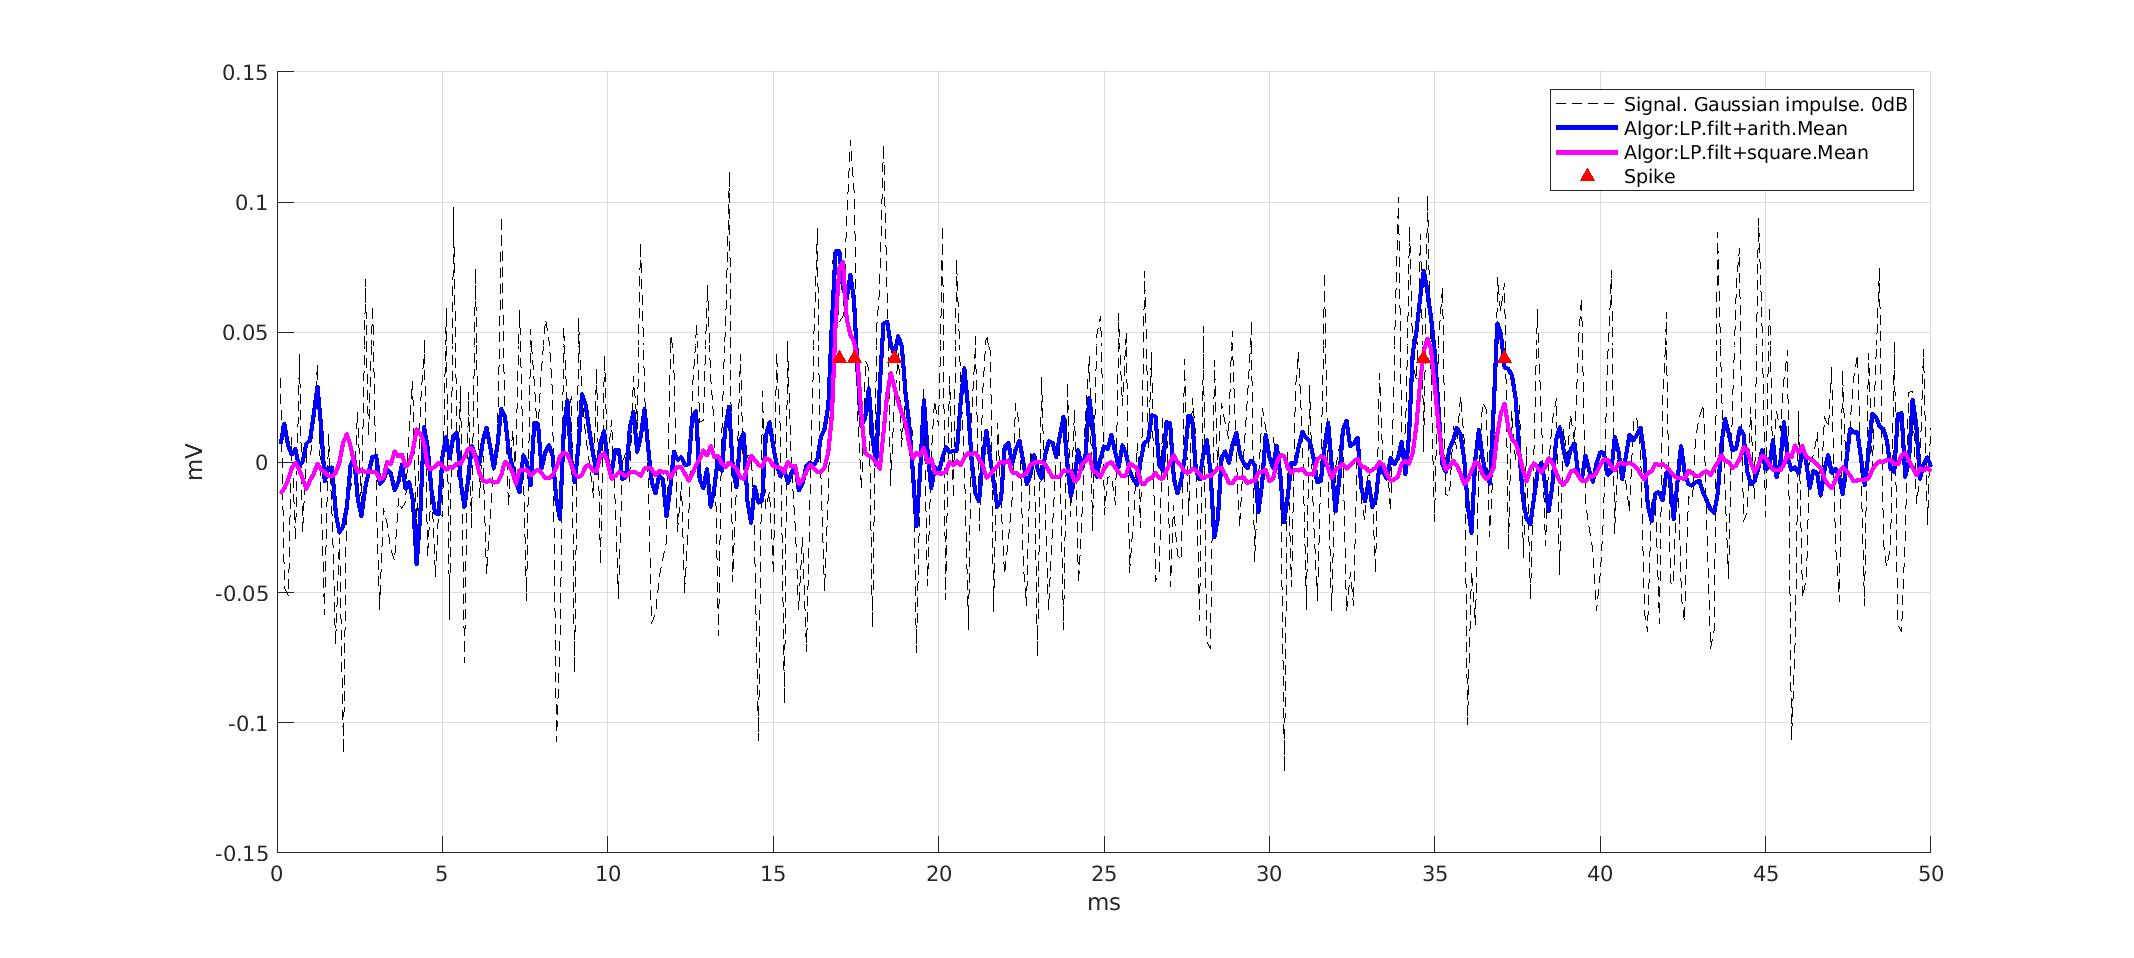
\includegraphics[width=2\linewidth]{results/c1_I2SNR0time.jpg}
\includegraphics[width=2\linewidth]{Graph/time.jpg}
\caption{Serie temporali. Segnale e filtri. Impulso gaussiano}
\label{fig:c1_I2SNR0time}
\end{figure}

%\begin{figure}[htbp]
%\centering
%\includegraphics[width=1\linewidth]%{results/c1_I4SNR0time.jpg}
%\caption{Serie temporali. Segnale e %filtri. Impulso spike}
%\label{fig:c1_I4SNR0time}
%\end{figure}




\section{Metriche di valutazione degli algoritmi}

Sotto il profilo spettrale, un buon filtro trasforma uno spettro rumoroso in modo da far emergere i picchi delle frequenza caratteristiche del segnale (toni) rispetto al rumore di fondo.
%
Nel contesto della presenza simulazione, dove il segnale è composto da impulsi di data forma funzionale, non necessariamente sinusoidale e di durata limitata, si deve tener conto anche di una visione {\it timbrica}, in cui rileva anche la forma caratteristica dei picchi e dello spettro in generale, forme che riflettono sia la forma funzionale degli impulsi sia le diverse irregolarità introdotte nel segnale.
%
In questo senso, un buon filtro dovrebbe restiture uno spettro del segnale rumoroso filtrato quanto più vicino a quello del segnale non rumoroso.
La metrica che valuta la distanza spettrale adottata in questo lavoro è presentata nel paragrafo \ref{metricaS}.

Sotto il profilo temporale invece, un buon algoritmo azzera il segnale dove non rileva impulsi in modo da ridurre gli errori di previsione di un test di soglia come il seguente
\begin{equation*}
t = t_{spike} \Leftrightarrow V(t) > V_{treshold}
\end{equation*}
Per test di soglia si intende perciò un criterio di discriminazione degli impulsi che si basa esclusivamente sull'ampiezza del segnale filtrato: scelto un valore di riferimento per il massimo rumore ammesso, tutti i punti del segnale sopra tale soglia si marcano come impulsi e come rumore il resto.
Tale procedura è chiaramente soggetta ad errore, la cui quantificazione 
attraverso opportune metriche da luogo alla valutazione di accuratezza dell'algoritmo adottato. In questo lavoro, la capacità predittiva degli algoritmi di sorting è valutata con la metrica illustrata nel paragrafo \ref{metricaT}.

Come illustrato nel paragrafo \ref{risultati}, le due metriche adottate sono fortemente correlate e l'analisi della loro congiunta distribuzione al variare del $SNR$ e della forma degli impulsi permette di valutarne la coerenza.



\subsection{Distanza spettrale}
\label{metricaS}

La distanza spettrale considerata è la distanza euclidea tra gli spettri nella banda $[0-\nu_{high}]$, dove $\nu_{high}$ è la frequenza alta di taglio del filtro passa banda.
% 
Nella formula che segue $DFT_{ref}$ è lo spettro del segnale di riferimento, non rumoroso e $DFT_{noisy.filt}$ quella del segnale rumoroso dopo essere stato soggetto agli algoritmi di sorting.
%
\begin{align*}
 d_{s}^2 & = \sum_{j:0}^{\nu_{high}}(DFT_{ref}(j) - DFT_{noisy.filt}(j) )^2
\end{align*}
%
L'indice $j$ corre solo nelle frequenze della banda di interesse, tenuto conto dei parametri di simulazione.




\subsection{Errore medio di previsione}
\label{metricaT}

Nel segnale di prova di riferimento sono noti i tempi di emissione degli impulsi.
%
Nel segnale filtrato questo tempo è incerto a causa dell'effetto congiunto della fase del filtro, della rumorosità del segnale e dell'azione dell'algoritmo.
%
La valutazione dell'errore medio di previsione è condotta con l'algoritmo \ref{alg:errore} nella seguente tabella. In breve, presi tutti e soli gli impulsi rilevati, ovvero i primi $N$ picchi più alti del segnale filtrato, l'algoritmo determina per ogni impulso rilevato quale sia il più vicino impulso reale e registra la differenza in termini di numero di campioni tra il momento dell'impulso rilevato e quello dell'impulso più vicino, in valore assoluto. L'errore complessivo viene infine riportato in $ms$ e in misura media su tutti gli $N$ impulsi.

\begin{algorithm}
\caption{Calcolo errore medio di previsione}\label{alg:errore}
\begin{algorithmic}[1]
%\Procedure{Euclid}{$a,b$}\Comment{The g.c.d. of a and b}
\State $t_{j=1,...,N}$ \Comment{Noti gli N tempi nel segnale di riferimento}
\State $\tau_{j=1,...,N}$ \Comment{Estraggo i primi N massimi nel segnale filtrato}
\State $\tau_{j}\mapsto d_{j} = min( |t_{1}-\tau_{j}|, |t_{2}-\tau_{j}|, ...)$ \Comment{Ad ogni previsione associo la minima distanza con l'insieme dei veri tempi $t_{j}$}
\State $\sum_{1}^{N} d_{j}/N$ \Comment{Errore medio in $ms$}
%\State $f_{t}\gets \sum_{i=1:3} f_{t-i}/3$
% \EndWhile\label{euclidendwhile}
% \State \textbf{return} $b$\Comment{The gcd is b}
% \EndProcedure
\end{algorithmic}
\end{algorithm}

Questa semplice metrica ha natura esplorativa ed è da intendersi solo indicativa della bontà di previsione, e viene utilizzata in questo lavoro solo per l'analisi esplorativa nei grafici di dispersione presentati qui di seguito. In particolare si evidenzia che la metrica non rileva in alcun modo la presenza di previsioni multiple sullo stesso impulso o la presenza di impulsi non rilevati.

% \begin{figure}[htbp]
% \centering
% \includegraphics[width=1\linewidth]{Graph/disegno.jpg}
% \caption[Disegno esemplificativo della classificazione delle previsioni]{Disegno esemplificativo della classificazione delle previsioni. Gli impulsi previsti $\tau_{j}$, $j=1,..,4$ sono determinati dall'intersezione della linea di soglia in grigio con il segnale filtrato (linea superiore). Gl intervalli temporali interessati da impusi effettivi sono invece indicati dai rettangoli lungo la linea sottostante. Le linee in rosso indicano gli sfasamenti temporali considerati nel calcolo dell'errore medio di previsione del primo algoritmo. In questo esempio, il secondo algoritmo conta invece due impulsi previsti, al tempo $t_{2}$ e $t_{4}$, due impulsi non rilevati al tempo $t_{1}$ e $t_{3}$ e due corrispondenti falsi positivi. Risultano correttamente previsti inoltre tutti i tempi d'attesa, ad eccezione del primo intervallo.
% 
% L'esempio evidenza come sia possibile che più rilevazioni insistano sullo stesso impulso emesso oppure che, a causa della soglia in ampiezza fissata, alcuni impulsi emessi non siano rilevati (impulso $t_{3}$)}
% \label{fig:scatter1}
% \end{figure}

Per completare l'analisi della capacità previsivia dei test, si utilizza invece un indicatore più formale. Qui di seguito illustrato nell'algoritmo \ref{alg:matrice}.

\begin{algorithm}
\caption{Calcolo errore medio di previsione}\label{alg:matrice}
\begin{algorithmic}[1]

%\Procedure{Euclid}{$a,b$}\Comment{The g.c.d. of a and b}
\State $t_{j=1,...,N}$ \Comment{Noti gli N tempi nel segnale di riferimento}
\State $\tau_{j=1,...,N}$ \Comment{Estraggo i primi N massimi nel segnale filtrato}
\State $\tau_{j}\mapsto d_{j} = min( |t_{1}-\tau_{j}|, |t_{2}-\tau_{j}|, ...)$ \Comment{Ad ogni previsione associo la minima distanza con l'insieme dei veri tempi $t_{j}$}
\State Se $d_{j}<\frac{D}{2}$ \Comment{Se l'errore è minore della semidurata degli impulsi allora la previsione si intende corretta. L'impulso viene marcato come rilevato, se già non lo era da una precedente previsione.}
\State Se $d_{j}>\frac{D}{2}$ \Comment{Se l'errore è maggiore della semidurata degli impulsi allora la previsione si intende errata. L'evento viene marcato come un falso positivo, se già non lo era da una precedente previsione.}
\State  \Comment{Il numero di falsi negativi si determina per differenza di $N$ con gli impulsi rilevati.}
\State  \Comment{Il numero di veri negativi si determina per differenza di $N$ con il numero di falsi positivi.}

\end{algorithmic}
\end{algorithm}

In breve, data una media di $150$ impulsi in un segnale della durata di $1s$, l'algoritmo registra gli impulsi rilevati e determina quelli non rilevati per differenza. La registrazione è dicotomica, non si contano cioè il numero di previsioni che rilevano lo stesso impulso. Simmetricamente, il segnale può essere scomposto in $150$ spazi vuoti che rappresentano i tempi di attesa tra due impulsi. L'algoritmo conta gli spazi vuoti che ricevono una previsione di impulso e determina così i falsi positivi e, per differenza, i veri negativi.

L'applicazione di questo algoritmo riassume tutta la simulazione in una matrice $2x2$ che rappresenta la distribuzione congiunta dei tempi di emissione previsti e di quelli effettivi. Maggiori sono gli elementi concordanti della matrice, quelli cioè posti sulla diagonale principale, dove a impulsi effettivi corrispondono impulsi previsti e viceversa, maggiore sarà la bontà dell'algoritmo.

Si osserva che nell'applicazione di questo algoritmo è implicita una tolleranza nella previsione del tempo d'impulso pari alla durata dell'impulso stesso.

Infine, dati i parametri di simulazione utilizzati, la lunghezza di un impulso che è di $9$ campioni e la distanza media tra gli impulsi di $60$ campioni, un algoritmo casuale di rilevazione ha una matrice degli errori caratteristica basata sul {\it fattore casuale di successo} di $\frac{9}{60}$ di cui bisogna tener conto in sede di valutazione dei risultati. 




\chapter{Risultati}
\section{Andamento degli errori di previsione}
\label{risultati}

I grafici \ref{fig:scatter1} $-$ \ref{fig:scatter5} mostrano la distribuzione congiunta delle metriche temporale e spettrale. Come atteso, si evidenzia (1) una forte correlazione positiva tra le due metriche, (2) l'andamento crescente con il decrescere del $SNR$, (3) una distinta collazione dei punti in base all'algoritmo di sorting e al tipo di impulso.

Per quanto riguarda gli impulsi rettangolare e gaussiano si evidenziano due fasi. La prima con $SNR$ fino a $-12$ $dB$, l'errore medio di previsione mostra un andamento simile per le due categorie di test, quadratico e semplice, se non addirittura favorevole al test quadratico. Poi per $SNR$ inferiori, si evidenzia una marcata divergenza delle performance dei test a media quadratica, come se l'aumento della rumorosità avesse l'effetto congiunto di distorcere lo spettro e peggiorare la precisione con cui si determinano i momenti degli impulsi. L'andamento delle due metriche è concorde, come previsto. Per quanto riguarda l'impulso sinusoidale si evidenzia invece una netta separazione nelle performance previsive dei due algoritmi.

Tuttavia ciò che indebolisce l'evidenza riportata da questi grafici è il valore medio della distanza temporale, mai superiore a $1$ $ms$; sebbene l'andamento sia peggiorativo con l'$SNR$, l'errore di previsione medio non è mai superiore alla semidurata degli impulsi. Tale considerazione fa sospettare che le {\it differenze visive di natura grafica} siano dovute esclusivamente alla differenza di rilevazione del centro dell'impulso, indotte dalla diversa forma funzionale. In particolare, impulsi simmetrici (gaussiano, rettangolare) vengono meglio rilevati rispetto a quelli asimmetrici (sinusoidale, neurale). Risulta a questo punto necessaria un'analisi più approfondita.


\begin{figure}[htbp]
\centering
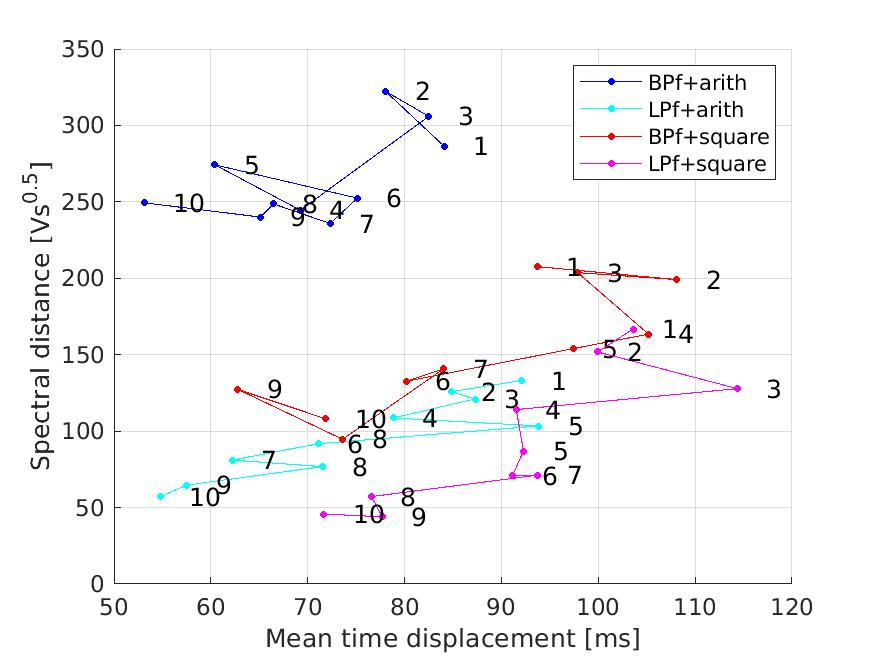
\includegraphics[width=1\linewidth]{Graph/scatter1.jpg}
\caption[Distribuzione congiunta delle metriche di valutazione al variare dell'SNR: impulso rettangolare]{Distribuzione congiunta delle metriche di valutazione: impulso rettangolare. $SNR$ da $-3$, a $-14$ dB. Le linee a toni blu sono relative al test semplice in media aritmetica, in toni rossi quelle del test quadratico.}
\label{fig:scatter1}
\end{figure}

\begin{figure}[htbp]
\centering
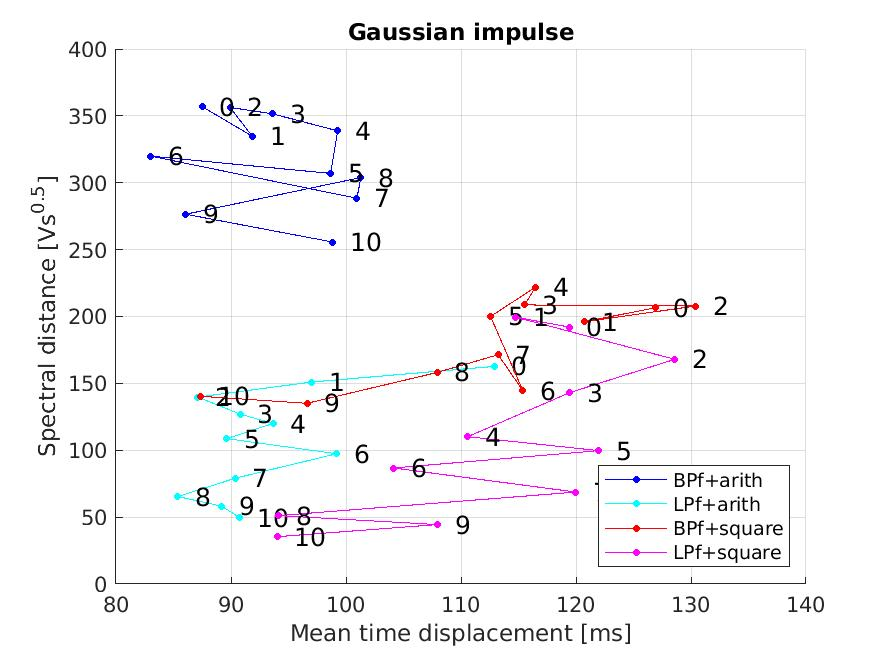
\includegraphics[width=1\linewidth]{Graph/scatter2.jpg}
\caption[Distribuzione congiunta delle metriche di valutazione al variare dell'SNR: impulso gaussiano ]{Distribuzione congiunta delle metriche di valutazione: impulso gaussiano. $SNR$ da $-3$, a $-14$ dB. Le linee a toni blu sono relative al test semplice in media aritmetica, in toni rossi quelle del test quadratico.}
\label{fig:scatter2}
\end{figure}

\begin{figure}[htbp]
\centering
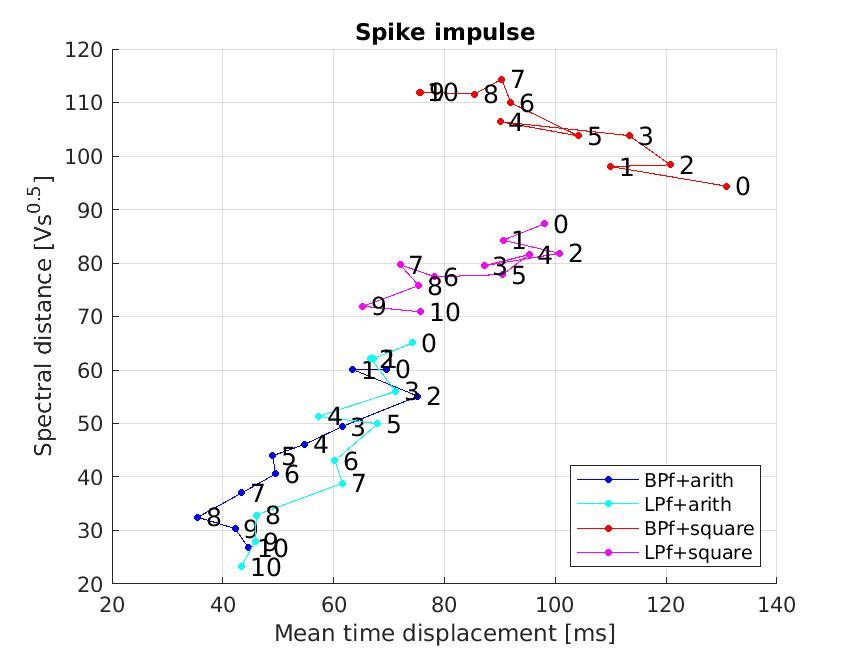
\includegraphics[width=1\linewidth]{Graph/scatter4.jpg}
\caption[Distribuzione congiunta delle metriche di valutazione al variare dell'SNR: impulso neurale ]{Distribuzione congiunta delle metriche di valutazione: impulso neurale. $SNR$ da $-3$, a $-14$ dB. Le linee a toni blu sono relative al test semplice in media aritmetica, in toni rossi quelle del test quadratico.}
\label{fig:scatter4}
\end{figure}

\begin{figure}[htbp]
\centering
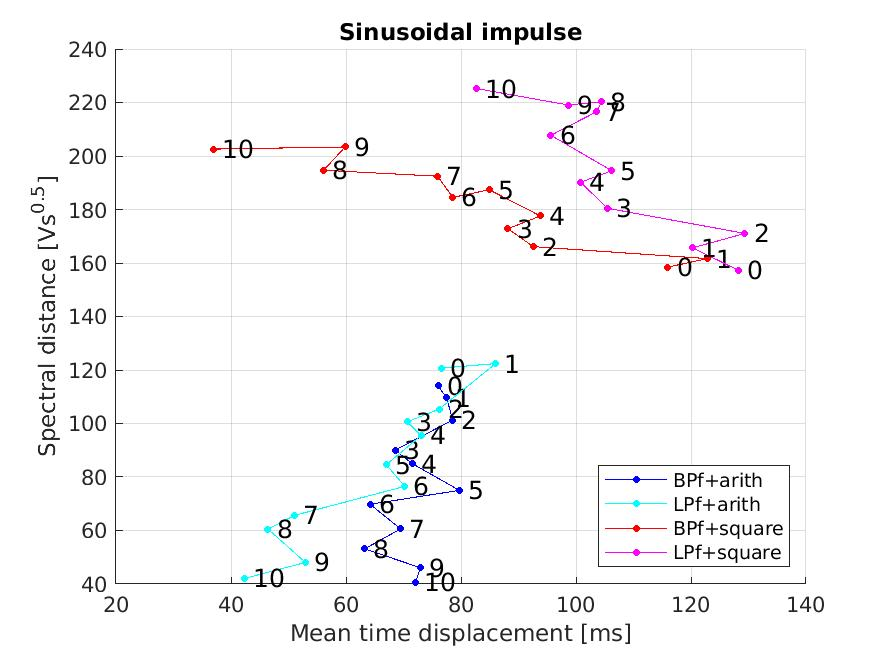
\includegraphics[width=1\linewidth]{Graph/scatter5.jpg}
\caption[Distribuzione congiunta delle metriche di valutazione al variare dell'SNR: impulso sinusoidale ]{Distribuzione congiunta delle metriche di valutazione:: impulso sinusoidale. $SNR$ da $-3$, a $-14$ dB. Le linee a toni blu sono relative al test semplice in media aritmetica, in toni rossi quelle del test quadratico.}
\label{fig:scatter5}
\end{figure}



%-----------------------------------------
%-----------------------------------------
%-----------------------------------------
\section{Valutazione di accuratezza delle previsioni}
\label{accuratezza}


\subsection{Indici di accuratezza}
\label{indici}
Nella tabella \ref{tab:indici} i filtri preliminari in frequenza sono indicati con
$BP$: passa banda,
$LP$: passa basso.
I test invece con
$1$: semplice, a media aritmetica, il test di riferimento.
$2$: quadratico, il test in potenza in valutazione.

Il valore numerico degli indici in tabella evidenzia la superiorità dei test in tensione a media semplice, con indici di concorcadanza medi sempre superiori ai test a media quadratica.

\begin{table}[htbp]
\centering
\caption[Indici di accuratezza: tasso di rilevazione, indice di Jaccard e F1 score]{\bf Indici di accuratezza}
\begin{tabular}{ccccc}
\hline
%Test              & \multirow{2}{}{Semplice} & \multirow{2}{}{Quadratico} \\
Test                & BP-1 & BP-2 & LP-1 & LP-2 \\
\hline
& & & & \\
Tasso di rilevazione & 0.55      &0.32      &0.54      &0.32\\
Punteggio F1         & 0.3384    &0.2159    &0.3349    &0.2211\\
Indice di Jaccard    & 0.7336    &0.5795    &0.7281    &0.5886 \\
& & & & \\
\hline
\end{tabular}
\label{tab:indici}
\end{table}


\subsection{Matrici di accuratezza}
\label{matrici}

Il dettaglio delle matrici di accuratezza da cui sono stati calcolati gli indici al paragrafo \ref{indici} è qui di seguito riportato.

%
\begin{table}[htbp]
\centering
\begin{tabular}{cccclcc}
                           &                         & \multicolumn{2}{c}{BP-1}                           &                       & \multicolumn{2}{c}{BP-2}                           \\
                           &                         & \multicolumn{2}{c}{Previsto}                       &                       & \multicolumn{2}{c}{Previsto}                       \\
                           &                         & si                      & no                       &                       & si                      & no                       \\ \cline{3-4} \cline{6-7} 
\multirow{2}{*}{Effettivo} & \multicolumn{1}{c|}{si} & \multicolumn{1}{c|}{83} & \multicolumn{1}{c|}{67} & \multicolumn{1}{l|}{} & \multicolumn{1}{c|}{48} & \multicolumn{1}{c|}{102} \\ \cline{3-4} \cline{6-7} 
                           & \multicolumn{1}{c|}{no} & \multicolumn{1}{c|}{13} & \multicolumn{1}{c|}{137} & \multicolumn{1}{l|}{} & \multicolumn{1}{c|}{24} & \multicolumn{1}{c|}{126} \\ \cline{3-4} \cline{6-7} 
                           &                         &                         &                          &                       &                         &                          \\
                           &                         & \multicolumn{2}{c}{LP-1}                           &                       & \multicolumn{2}{c}{LP-2}                           \\
                           &                         & \multicolumn{2}{c}{Previsto}                       &                       & \multicolumn{2}{c}{Previsto}                       \\
                           &                         & si                      & no                       &                       & si                      & no                       \\ \cline{3-4} \cline{6-7} 
Effettivo                  & \multicolumn{1}{c|}{si} & \multicolumn{1}{c|}{82} & \multicolumn{1}{c|}{68} & \multicolumn{1}{l|}{} & \multicolumn{1}{c|}{49} & \multicolumn{1}{c|}{101} \\ \cline{3-4} \cline{6-7} 
                           & \multicolumn{1}{c|}{no} & \multicolumn{1}{c|}{14} & \multicolumn{1}{c|}{136} & \multicolumn{1}{l|}{} & \multicolumn{1}{c|}{22} & \multicolumn{1}{c|}{128} \\ \cline{3-4} \cline{6-7} 
\end{tabular}
\caption[Distribuzione congiunta degli impulsi emessi e rilevati. Matrice di accuratezza.]{\bf Matrici di accuratezza}
\label{tab:matrici}
\end{table}
%




\section{Riepilogo}
\label{conclusioni}

Con questa simulazione si è voluto verificare il comportamento di un algoritmo di rilevazione degli impulsi neurali comunemente utilizzato in letteratura \cite{Lambacher2011}, in un contesto di alta rumorosità e irregolarità del segnale. I segnali neurali sono impulsi in tensione caratterizzati dall'alternanza di una fase di alta tensione positiva con una fase in cui la tensione si sposta verso valori negativi e per questo si rende conveniente l'utilizzo di tecniche di elaborazione del segnale che ne considerano la potenza trasmessa, e che ad un certo stato dell'elaborazione trasformano il segnale elevandolo al quadrato. Risultato di questo tipo di elaborazione è idealmente un segnale di piccola intensità nei tempi d'attesa tra due impulsi contigui e di elevata intensità negli intervalli in cui si manifestano gli impulsi, rendendo così agevole la loro rilevazione.

La procedura di elaborazione suddetta può presentare delle difficoltà applicative nel contesto degli esperimenti di rilevazione con tecnologia $MEA$, in cui si inserisce questo lavoro, a causa sia dell'elevata rumorosità del segnale, che della forma ignota degli impulsi. Inoltre la procedura di elaborazione basata sulla potenza del segnale non permette di sfruttare appieno l'elevata densità spaziale dei sensori, grazie alla quale una stessa cellula neurale e il relativo segnale emesso, può essere campionato da più sensori in diverse posizioni.

Al fine di verificare il comportamento delle procedure di elaborazione del segnale in potenza nel contesto della tecnologia $MEA$ questo lavoro simula un segnale altamente rumoroso rilevato da un cluster di sensori contigui e ne confronta gli errori di previsione con una procedura di elaborazione del segnale in tensione, che tra le varie trasformazione esegue una media aritmentica spaziale tra i pixel che campionano una stessa cellula neurale. L'idea sottostante a questa procedura di riferimento è che lo stesso segnale possa essere rilevato da più sensori e quindi pulito da un aparte di rumore con l'elaborazione di un segnale medio.


\section{Raffronto: elaborazione del segnale in potenza e in tensione}
A priori, sono diverse le considerazioni che si possono muovere a sfavore dell'efficacia degli algoritmi di rilevazione basati sulla potenza del segnale in un contesto di alta rumorosità e irregolarità degli impulsi. In primo luogo, l'applicazione del quadrato non permette di sfruttare l'elevata frequenza di campionamento spazio temporale per mediare segnali da pixel diversi e ridurre così compensativamente il rumore. In secondo luogo, laddove gli impulsi sono irregolari e limitati nel tempo l'applicazione di una trasformazione non lineare ad un pacchetto di frequenze comporta distorsioni allo spettro facendo comparire, in seguito all'elevamente al quadrato, picchi spettrali che non sono invece presenti nel segnale originale. D'altro canto, i test a media semplice non inducono alcuna distorsione spettrale e permettono di mediare il rumore tra diversi pixel. A sfavore dei test in tensione a media semplice, si può invece argomentare che in presenza di impulsi a media nulla, con parti positive e negative, una delle due non può essere utilizzata per rilevare gli impulsi con test di soglia.
%
I risultati qui esposti dimostrano che le distorsioni spettrali introdotte dai test a media quadratica, il comparire cioè di picchi in frequenza non presenti nello spettro originale a causa dell'elevamento al quadrato, sebbene non risultino visibili graficamente, in quanto smorzati dall'irregolarità del segnale, sono comunque rilevati dalla metrica di distanza spettrale e contribuiscono a deteriorare la capacità previsiva di questa categoria di test.
%
I test a media semplice, per contro, risultano molto precisi sia nella sagoma spettrale restituita, sia nella rilevazione del tempo degli impulsi. Inoltre, l'insieme degli impulsi correttamente rilevati da questi test è maggiore rispetto a quello dei test a media quadratica, come evidenziato dai conteggi riportati nelle matrici di errore.
%
Le risultanze intermedie dei grafici di andamento congiunto vengono periò confermate. Sebbene le differenze grafiche visive siano da attribuire a differenze nella rilevazione del centro dell'impulso, in funzione delle diverse forme funzionali degli impulsi utilizzati, l'andamento crescente dell'errore di previsione è effettivamente indicativo del deterioramento delle capacità previsive dei test a media quadratica, sebbene i valori di errore medio siano molto bassi. Circostanza che si spiega per l'elevata percentuale di impulsi correttamente previsti, che abbassa i valori dell'errore medio di entrambe le categorie di test.



\section{Conclusioni}
La simulazione proposta evidenzia che per sfruttare l'elevata densità spaziale dei sensori 
della tecnologia $MEA$, grazie alla quale una stessa cellula neurale e il relativo segnale emesso può essere campionato da più sensori in diverse posizioni, le procedure di elaborazione del segnale in potenza dovrebbero essere applicate solo successivamente alla riduzione del rumore, utilizzando delle medie spaziali sui diversi rilevatori che campionano la stessa fonte di emissione degli impulsi.

Secondo questa procedura di elaborazione del segnale, la prima fase di elaborazione si focalizzerebbe sul segnale in tensione e non apporterebbe distorsioni allo spettro del segnale emesso. In questa prima fase lo spettro del segnale è ancora utilizzabile per verificare le proprietà della fonte emissiva degli impulsi. In un seconda fase, una volta che il segnale è stato pulito da una parte del rumore grazie all'effetto compensativo delle medie spaziali sul rumore di tipo {\it white noise}, i test in potenza risultano il modo più appropriato per trasformare il segnale grezzo in un indicatore di impulsi.


\section{Ulteriori prospettive di indagine}
I risultati qui esposti si basano sulla possibilità di elaborare un segnale medio derivante dai diversi segnali dei sensori che campionano la stessa cellula emettitrice di impulsi. La qualità del segnale medio in questa simulazione è sempre migliore di quello grezzo grazie alle caratteristiche ideali del rumore utilizzato: rumore additivo di variabili casuali indipendenti e identicamente distribuite. 
La presente simulazione non prende perciò in considerazione due aspetti che possono essere validi nel contesto sperimentale di riferimento: (1) la propagazione del segnale e (2) la correlazione del rumore. Entrambi sono in particolare  legati alla presenza di una soluzione fisiologica in cui le cellule neurali sono immerse. Il primo aspetto, quello della propagazione del segnale, potrebbe impattare sui risultati della presente simulazione solo qualora la propagazione dell'impulso tra pixel contigui induca una sovrapposizione distruttiva del segnale: la media aritmetica tra pixel diversi risulterebbe in una complessiva riduzione dell'intensità del segnale se pixel contigui campionano fasi di tensione di impulso di segno opposto. Il secondo aspetto invece, renderebbe inutile l'applicazione della media spaziale, non potendosi concretizzare completamente l'abbattimento della varianza del rumore.



\backmatter


\include{biblio.bib}

% Do not use this command if you did not prepare a nomenclature
% database by means od the suitable \nomenclature command and its
% arguments, as we did in chapter 2 of this example thesis.
\printnomencl

% In this example we use \nocite{*} in order to typeset the whole
% contents of the bibliographic database. Normally this is not
% necessary and it's better to let biber extract from the database
% only the cited works
\nocite{*}


\printbibliography[heading=bibintoc]

% Do not use this command if you did not set the \makeindex switch
% in the preamble.

\printindex

\end{document}

